\documentclass[a4paper, 11pt, oneside]{scrartcl}

% --- Pacchetti Fondamentali ---
\usepackage[utf8]{inputenc}
\usepackage[T1]{fontenc}
\usepackage[italian]{babel}
\usepackage{lmodern}
\usepackage{array}
\usepackage{colortbl}
\usepackage{longtable}
\usepackage{float}
\usepackage{scrhack}
\usepackage{placeins}
\usepackage{tabularx}
\usepackage{amsmath, amssymb, mathtools}

% --- Grafica e Layout ---
\usepackage{graphicx}
\graphicspath{{Contenuti/}{../../assets/}{../assets/}{assets/}}
\usepackage[a4paper, top=2.5cm, bottom=3cm, left=2.5cm, right=2.5cm]{geometry}
\usepackage{fancyhdr}
\usepackage{microtype}
\usepackage[svgnames,table]{xcolor}

% --- Utility ---
\usepackage{booktabs}
\usepackage{enumitem}
\usepackage{hyperref}
\usepackage{caption}
\usepackage{hhline}
\usepackage[italian]{cleveref}
\usepackage{listings}

\hypersetup{
    colorlinks=true,
    linkcolor=DarkBlue,
    filecolor=DarkBlue,
    urlcolor=DarkBlue,
    citecolor=DarkBlue,
    pdftitle={Specifica Tecnica - NightPRO},
    pdfauthor={Gruppo NightPRO},
}

% --- Colonne tabella personalizzate ---
\newcolumntype{L}{>{\raggedright\arraybackslash}X}
\newcolumntype{R}{>{\raggedleft\arraybackslash}X}
\newcolumntype{C}{>{\centering\arraybackslash}X}

% --- Stile codice ---
\lstset{
    basicstyle=\ttfamily\small,
    breaklines=true,
    frame=single,
    backgroundcolor=\color{gray!5},
    rulecolor=\color{gray!40},
    numbers=left,
    numberstyle=\tiny\color{gray},
    keywordstyle=\color{DarkBlue}\bfseries,
    stringstyle=\color{OrangeRed},
    commentstyle=\color{ForestGreen}\itshape,
    showstringspaces=false,
    tabsize=2
}

% ===================================================================
%  HEADER E FOOTER
% ===================================================================
\pagestyle{fancy}
\fancyhf{}
\fancyhead[L]{\textbf{NightPRO -- Progetto Ingegneria del Software}}
\fancyhead[R]{Anno Accademico 2025/2026}
\fancyfoot[C]{\thepage}
\renewcommand{\headrulewidth}{0.4pt}
\renewcommand{\footrulewidth}{0.4pt}

\setcounter{secnumdepth}{5}
\setcounter{tocdepth}{4}

% ===================================================================
%  INIZIO DOCUMENTO
% ===================================================================
\begin{document}

% -------------------------------------------------------------------
%  FRONTESPIZIO
% -------------------------------------------------------------------
\thispagestyle{empty}
\begin{titlepage}
    \centering
    \vspace*{1cm}
    %
\includegraphics[width=0.35\textwidth]{logo.png}\\[1cm]

    \vfill

    {\small UNIVERSIT\`A DEGLI STUDI DI PADOVA \par}
    {\small CORSO DI LAUREA IN INFORMATICA (L-31) \par}
    \vspace{0.5cm}
    {\large Corso di Ingegneria del Software \par}
    {\small Anno Accademico 2025/2026 \par}
    \vfill

    {\Huge \bfseries Specifica Tecnica \par}
    \vspace{1cm}

    \vfill

    {\Large \bfseries Gruppo: NightPRO}    \vspace{0.5cm}\\
    {\Large \bfseries Sistema: SmartOrder}    \vspace{0.5cm}

    {\large \href{mailto:swe.nightpro@gmail.com}{swe.nightpro@gmail.com}}\\[2cm]

    {\large Data: 2026-03-31 \par}

    {\Large Versione: 0.3\par}

\end{titlepage}

% -------------------------------------------------------------------
%  TABELLA DELLE VERSIONI
% -------------------------------------------------------------------
\newpage
\pagestyle{fancy}
\phantomsection
\section*{Tabella delle Versioni}
\vspace{0.2cm}
\begin{center}
    \resizebox{\textwidth}{!}{
        \renewcommand{\arraystretch}{1.2}
        \begin{tabular}{@{}llp{0.25\textwidth}p{0.45\textwidth}c@{}}
            \toprule
            \textbf{Versione} & \textbf{Data} & \textbf{Autore/i} & \textbf{Descrizione delle Modifiche}                           & \textbf{Verificatore} \\
            \midrule
            0.3               & 2026-03-31    & D. Biasuzzi, F. Zanella, S. Perozzo    & Riorganizzazione documento, inserimento dei diagrammi PlantUML e stesura delle sezioni 4, 5, 6 e 7 & M. M. Romascu\\
            0.2               & 2026-03-26    & Davide Biasuzzi   & Inserimento paragrafo su esecuzione e su tecnologie utilizzate & Leonardo Bilato       \\
            0.1               & 2026-03-20    & Davide Biasuzzi   & Stesura base documento (Introduzione e Requisiti di Sistema)   & Leonardo Bilato       \\
            \bottomrule
        \end{tabular}
    }
\end{center}

% -------------------------------------------------------------------
%  INDICE
% -------------------------------------------------------------------
\newpage
\tableofcontents
\listoffigures
\listoftables
\pagestyle{fancy}

% -------------------------------------------------------------------
%  COMPONENTI DEL GRUPPO
% -------------------------------------------------------------------
\newpage
\section*{Componenti del Gruppo}
\addcontentsline{toc}{section}{Componenti del Gruppo}

\begin{table}[H]
    \centering
    \renewcommand{\arraystretch}{1.2}
    \begin{tabular}{@{}llc@{}}
        \toprule
        \textbf{Cognome} & \textbf{Nome}   & \textbf{Matricola} \\
        \midrule
        Biasuzzi         & Davide          & 2111000            \\
        Bilato           & Leonardo        & 2071084            \\
        Zanella          & Francesco       & 2116442            \\
        Romascu          & Mihaela-Mariana & 2079726            \\
        Ogniben          & Michele         & 2042325            \\
        Perozzo          & Samuele         & 2110989            \\
        Ponso            & Giovanni        & 2000558            \\
        \bottomrule
    \end{tabular}
    \caption{Componenti del gruppo NightPRO.}
\end{table}

% ===================================================================
%  1. INTRODUZIONE
% ===================================================================
\newpage
\section{Introduzione}

\subsection{Scopo del documento}
Il presente documento ha lo scopo di descrivere l'architettura software del sistema \textit{SmartOrder}, definendo le scelte tecnologiche, i pattern architetturali e progettuali adottati, e l'architettura di dettaglio di ciascun componente.
La Specifica Tecnica costituisce il riferimento principale per la fase di codifica, garantendo coerenza tra progettazione e implementazione.

\subsection{Scopo del prodotto}
\textit{SmartOrder} \`e una piattaforma B2B per l'automazione della gestione degli ordini commerciali. Il sistema consente ai clienti di formulare ordini in linguaggio naturale (testo, audio, immagini) e li converte automaticamente in ordini strutturati pronti per l'integrazione con sistemi ERP aziendali, riducendo errori e tempi di inserimento manuale.

\subsection{Glossario}
Per evitare ambiguit\`a, i termini tecnici e di dominio utilizzati nel documento sono definiti nel \textit{Glossario v2.0}.
I termini presenti nel glossario sono contrassegnati con il simbolo \textsubscript{\textsc{g}} alla prima occorrenza in ogni sezione.

\subsection{Riferimenti}

\subsubsection{Riferimenti normativi}
\begin{itemize}
    \item \href{https://swenightpro.github.io/Documentazione/docs/RTB/Documentazione%20Interna/Norme_di_Progetto_v2.0.pdf}{Norme di Progetto v2.0} (Ultima modifica 2026-03-20)
\end{itemize}

\subsubsection{Riferimenti informativi}
\begin{itemize}
    \item \href{https://swenightpro.github.io/Documentazione/docs/RTB/Documentazione%20Esterna/Glossario_v2.0.pdf}{Glossario v2.0} (Ultima modifica 2026-03-20)
    \item \href{https://swenightpro.github.io/Documentazione/docs/RTB/Documentazione%20Esterna/Piano_di_Qualifica_v1.0.pdf}{Piano di Qualifica v1.0} (Ultima modifica 2026-03-20)
    \item \href{https://nextjs.org/docs}{Next.js Documentation} (Ultima modifica 2026-03-20)
    \item \href{https://fastapi.tiangolo.com/}{FastAPI Documentation} (Ultima modifica 2026-03-20)
    \item \href{https://platform.openai.com/docs}{OpenAI API Documentation} (Ultima modifica 2026-03-20)
    \item \href{https://www.postgresql.org/docs/}{PostgreSQL Documentation} (Ultima modifica 2026-03-20)
    \item \href{https://www.math.unipd.it/~rcardin/swea/2022/Software%20Architecture%20Patterns.pdf}{Software Architecture Patterns, SWE 2025-2026} (Ultima modifica 2026-03-26)
    \item \href{https://www.math.unipd.it/~rcardin/swea/2022/Design%20Pattern%20Architetturali%20-%20Dependency%20Injection.pdf}{Dependency Injection, SWE 2025-2026} (Ultima modifica 2026-03-26)
    \item \href{https://www.math.unipd.it/~rcardin/swea/2022/Design%20Pattern%20Creazionali.pdf}{Design Pattern Creazionali, SWE 2025-2026} (Ultima modifica 2026-03-26)
    \item \href{https://www.math.unipd.it/~rcardin/swea/2022/Design%20Pattern%20Strutturali.pdf}{Design Pattern Strutturali, SWE 2025-2026} (Ultima modifica 2026-03-26)

\end{itemize}

% ===================================================================
%  2. AMBIENTE MINIMO
% ===================================================================
\newpage
\section{Ambiente minimo}

\subsection{Software minimo}
\begin{table}[H]
    \centering
    \renewcommand{\arraystretch}{1.2}
    \begin{tabularx}{\textwidth}{@{}lXl@{}}
        \toprule
        \textbf{Software} & \textbf{Descrizione}                                  & \textbf{Versione minima} \\
        \midrule
        Node.js           & Runtime JavaScript per l'esecuzione dell'applicazione & $\geq$ 20.0              \\
        npm               & Gestore pacchetti Node.js                             & $\geq$ 10.0              \\
        Python            & Interprete Python per il modulo AI                    & $\geq$ 3.11              \\
        pip               & Gestore pacchetti Python                              & $\geq$ 23.0              \\
        PostgreSQL        & Database relazionale                                  & $\geq$ 16                \\
        Browser web       & Chrome, Firefox, Safari, Edge                         & Ultime 2 versioni        \\
        \bottomrule
    \end{tabularx}
    \caption{Software minimo per il deployment.}
\end{table}

\subsection{Hardware minimo}
\begin{table}[H]
    \centering
    \renewcommand{\arraystretch}{1.2}
    \begin{tabularx}{\textwidth}{@{}lX@{}}
        \toprule
        \textbf{Componente} & \textbf{Requisito}                    \\
        \midrule
        CPU                 & Processore 64-bit, $\geq$ 2 core      \\
        RAM                 & $\geq$ 4 GB                           \\
        Spazio disco        & $\geq$ 5 GB                           \\
        Connessione di rete & Richiesta per accesso alle API OpenAI \\
        \bottomrule
    \end{tabularx}
    \caption{Hardware minimo richiesto.}
\end{table}

% ===================================================================
%  4. TECNOLOGIE UTILIZZATE
% ===================================================================
\newpage

\section{Tecnologie utilizzate}

In questa sezione vengono elencate le tecnologie adottate per lo sviluppo del sistema \textit{SmartOrder}. Per ciascuna tecnologia viene indicata la versione utilizzata, la motivazione della scelta e il contesto d'impiego nel progetto.

% -------------------------------------------------------------------
\subsection{Linguaggi di programmazione}
% -------------------------------------------------------------------

\subsubsection{TypeScript}
\begin{itemize}[noitemsep]
\item \textbf{Versione:} 5
\item \textbf{Documentazione ufficiale:} \href{https://www.typescriptlang.org/docs/}{TypeScript
 Documentation} (Ultima modifica 2026-03-26)
\item \textbf{Ambito:} Frontend
\item \textbf{Contesto di utilizzo:} linguaggio principale per l'interfaccia utente dell'applicativo Next.js, sia per i componenti React che per la gestione dello stato lato client.
\item \textbf{Vantaggi:} tipizzazione statica che riduce errori a runtime, ottimo supporto IDE, compatibilit\`a nativa con React e Next.js.
\item \textbf{Svantaggi:} overhead di compilazione rispetto a JavaScript puro.
\end{itemize}

\subsubsection{Python}
\begin{itemize}[noitemsep]
\item \textbf{Versione:} 3.11
\item \textbf{Documentazione ufficiale:} \href{https://docs.python.org/3/}{Python 3 Documentation} (Ultima modifica 2026-03-26)
\item \textbf{Ambito:} Backend / Modulo AI
\item \textbf{Contesto di utilizzo:} implementazione della pipeline di elaborazione degli ordini tramite intelligenza artificiale e gestione delle API REST tramite FastAPI.
\item \textbf{Vantaggi:} ecosistema maturo in ambito NLP/ML, compatibilit\`a nativa con le librerie OpenAI, sintassi concisa, supporto asincrono con Uvicorn/ASGI.
\item \textbf{Svantaggi:} prestazioni inferiori a linguaggi compilati; mitigato dall'uso di Uvicorn (ASGI asincrono).
\end{itemize}

\subsubsection{SQL}
\begin{itemize}[noitemsep]
\item \textbf{Documentazione ufficiale:} \href{https://www.iso.org/standard/76584.html}{ISO/IEC 9075:2023 (SQL)} (Ultima modifica 2026-03-26)
\item \textbf{Ambito:} Database
\item \textbf{Contesto di utilizzo:} interrogazioni sul catalogo prodotti, gestione ordini, sessioni e carrelli.
\end{itemize}

% -------------------------------------------------------------------
\subsection{Framework e librerie}
% -------------------------------------------------------------------

\subsubsection{Next.js}
\begin{itemize}[noitemsep]
\item \textbf{Versione:} 15.5
\item \textbf{Documentazione ufficiale:} \href{https://nextjs.org/docs}{Next.js Documentation} (Ultima modifica 2026-03-26)
\item \textbf{Ambito:} Frontend full-stack
\item \textbf{Contesto di utilizzo:} framework principale per il frontend. Gestisce il rendering dell'interfaccia utente (React) e la logica lato client.
\item \textbf{Vantaggi:} App Router con Server Components, SSR e SSG, integrazione ottimale con React.
\item \textbf{Svantaggi:} curva di apprendimento per le convenzioni App Router; vincolo a React come libreria UI.
\end{itemize}

\subsubsection{React}
\begin{itemize}[noitemsep]
\item \textbf{Versione:} 19
\item \textbf{Documentazione ufficiale:} \href{https://react.dev/learn}{React Documentation} (Ultima modifica 2026-03-26)
\item \textbf{Ambito:} UI
\item \textbf{Contesto di utilizzo:} costruzione dell'interfaccia utente tramite componenti dichiarativi, gestione dello stato con Context API e Hooks.
\item \textbf{Vantaggi:} ecosistema vastissimo, modello a componenti riutilizzabili, Virtual DOM per aggiornamenti efficienti.
\end{itemize}

\subsubsection{Tailwind CSS}
\begin{itemize}[noitemsep]
\item \textbf{Versione:} 4.1
\item \textbf{Documentazione ufficiale:} \href{https://tailwindcss.com/docs}{Tailwind CSS Documentation} (Ultima modifica 2026-03-26)
\item \textbf{Ambito:} Styling
\item \textbf{Contesto di utilizzo:} stilizzazione dei componenti React con approccio utility-first.
\item \textbf{Vantaggi:} prototipazione rapida, design responsive\textsubscript{\textsc{g}} integrato, nessun CSS custom da mantenere.
\item \textbf{Svantaggi:} classi verbose nel markup; mitigato dalla composizione in componenti React.
\end{itemize}

\subsubsection{FastAPI}
\begin{itemize}[noitemsep]
\item \textbf{Versione:} 0.115
\item \textbf{Documentazione ufficiale:} \href{https://fastapi.tiangolo.com/}{FastAPI Documentation} (Ultima modifica 2026-03-26)
\item \textbf{Ambito:} Backend / Modulo AI
\item \textbf{Contesto di utilizzo:} espone gli endpoint \texttt{/chat} e \texttt{/transcribe} per l'elaborazione AI, gestione degli ordini e delle sessioni. Funziona come backend principale dell’applicazione.
\item \textbf{Vantaggi:} validazione automatica dei dati tramite Pydantic\textsubscript{\textsc{g}}, documentazione OpenAPI auto-generata, supporto nativo async/await.
\item \textbf{Svantaggi:} richiede un processo separato (Uvicorn) rispetto al runtime Node.js.
\end{itemize}

\subsubsection{Pydantic}
\begin{itemize}[noitemsep]
\item \textbf{Versione:} 2.9
\item \textbf{Documentazione ufficiale:} \href{https://docs.pydantic.dev/latest/}{Pydantic Documentation} (Ultima modifica 2026-03-26)
\item \textbf{Ambito:} Backend / Modulo AI
\item \textbf{Contesto di utilizzo:} definizione dei modelli di request/response per le API FastAPI, con validazione automatica dei tipi.
\end{itemize}

\subsubsection{OpenAI SDK}
\begin{itemize}[noitemsep]
\item \textbf{Versione:} 1.51
\item \textbf{Documentazione ufficiale:} \href{https://platform.openai.com/docs}{OpenAI API Documentation} (Ultima modifica 2026-03-26)
\item \textbf{Ambito:} Backend / Modulo AI
\item \textbf{Contesto di utilizzo:} SDK\textsubscript{\textsc{g}} ufficiale per l'integrazione con GPT-4o, GPT-4o-mini e Whisper.
\end{itemize}

% -------------------------------------------------------------------
\subsection{Strumenti di persistenza}
% -------------------------------------------------------------------

\subsubsection{PostgreSQL}
\begin{itemize}[noitemsep]
\item \textbf{Versione:} 16
\item \textbf{Documentazione ufficiale:} \href{https://www.postgresql.org/docs/16/}{PostgreSQL 16 Documentation} (Ultima modifica 2026-03-26)
\item \textbf{Ambito:} Database
\item \textbf{Contesto di utilizzo:} unica base dati del sistema, accessibile dal modulo AI tramite Python (\texttt{psycopg2}). Tutte le operazioni sul catalogo prodotti, ordini, sessioni e carrelli avvengono tramite FastAPI.
\item \textbf{Vantaggi:} robustezza, supporto a query complesse e full-text search, estensibilit\`a (pgvector per Vector Search\textsubscript{\textsc{g}}).
\end{itemize}

\subsubsection{psycopg2}
\begin{itemize}[noitemsep]
\item \textbf{Documentazione ufficiale:} \href{https://www.psycopg.org/docs/}{psycopg2 Documentation} (Ultima modifica 2026-03-26)
\item \textbf{Ambito:} Modulo AI / Backend
\item \textbf{Contesto di utilizzo:} driver Python per PostgreSQL con connection pooling\textsubscript{\textsc{g}} (\texttt{SimpleConnectionPool}).
\end{itemize}

% -------------------------------------------------------------------
\subsection{Intelligenza artificiale}
% -------------------------------------------------------------------

\subsubsection{GPT-4o}
\begin{itemize}[noitemsep]
    \item \textbf{Versione:} 2024-08-06
    \item \textbf{Documentazione ufficiale:} \href{https://platform.openai.com/docs/models/gpt-4o}{OpenAI GPT-4o} (Ultima modifica 2026-03-26)
    \item \textbf{Contesto di utilizzo:} modello linguistico principale per la comprensione degli ordini, la classificazione degli intenti e le decisioni di business. Utilizzato con temperature=0.1 per risposte deterministiche.
\end{itemize}

\subsubsection{GPT-4o-mini}
\begin{itemize}[noitemsep]
    \item \textbf{Documentazione ufficiale:} \href{https://platform.openai.com/docs/models/gpt-4o-mini}{OpenAI GPT-4o-mini} (Ultima modifica 2026-03-26)
    \item \textbf{Contesto di utilizzo:} modello leggero per l'estrazione rapida dei parametri di ricerca e la classificazione semantica degli intenti utente.
\end{itemize}

\subsubsection{Whisper}
\begin{itemize}[noitemsep]
    \item \textbf{Versione:} 1
    \item \textbf{Documentazione ufficiale:} \href{https://platform.openai.com/docs/guides/speech-to-text}{OpenAI Speech-to-Text (Whisper)} (Ultima modifica 2026-03-26)
    \item \textbf{Contesto di utilizzo:} trascrizione di messaggi audio in testo, con prompt specifico per il dominio Ergon e lingua forzata a italiano.
\end{itemize}

% -------------------------------------------------------------------
\subsection{Infrastruttura e DevOps}
% -------------------------------------------------------------------

\subsubsection{Docker}
\begin{itemize}[noitemsep]
    \item \textbf{Versione:} $\geq$ 24.0
    \item \textbf{Documentazione ufficiale:} \href{https://docs.docker.com/}{Docker Documentation} (Ultima modifica 2026-03-26)
    \item \textbf{Contesto di utilizzo:} containerizzazione dell'intero sistema per garantire portabilit\`a e riproducibilit\`a degli ambienti. Docker Compose ($\geq$ 2.20) orchestra l'avvio dei container.
\end{itemize}

\subsubsection{Node.js}
\begin{itemize}[noitemsep]
    \item \textbf{Versione:} 20
    \item \textbf{Documentazione ufficiale:} \href{https://nodejs.org/docs/latest-v20.x/api/}{Node.js 20 Documentation} (Ultima modifica 2026-03-26)
    \item \textbf{Contesto di utilizzo:} runtime JavaScript per l'esecuzione di Next.js in sviluppo e produzione.
\end{itemize}

\subsubsection{Uvicorn}
\begin{itemize}[noitemsep]
    \item \textbf{Versione:} 0.32
    \item \textbf{Documentazione ufficiale:} \href{https://www.uvicorn.org/}{Uvicorn Documentation} (Ultima modifica 2026-03-26)
    \item \textbf{Contesto di utilizzo:} server ASGI\textsubscript{\textsc{g}} per l'esecuzione di FastAPI, con supporto a richieste asincrone.
\end{itemize}

\subsubsection{GitHub Actions}
\begin{itemize}[noitemsep]
    \item \textbf{Documentazione ufficiale:} \href{https://docs.github.com/actions}{GitHub Actions Documentation} (Ultima modifica 2026-03-26)
    \item \textbf{Contesto di utilizzo:} pipeline di integrazione continua per quality checks (ESLint, build verification).
\end{itemize}

\subsubsection{ESLint}
\begin{itemize}[noitemsep]
    \item \textbf{Versione:} 9
    \item \textbf{Documentazione ufficiale:} \href{https://eslint.org/docs/latest/}{ESLint Documentation} (Ultima modifica 2026-03-26)
    \item \textbf{Contesto di utilizzo:} linter\textsubscript{\textsc{g}} statico per il codice TypeScript/JavaScript.
\end{itemize}



% ===================================================================
%  5. ARCHITETTURA DI SISTEMA
% ===================================================================
\newpage
%\input{Contenuti/architettura_monolitica}

% ===================================================================
%  6. ARCHITETTURA DI DEPLOYMENT
% ===================================================================
\newpage
\section{Architettura di sistema}
Questa sezione illustra l'architettura ad alto livello del sistema SmartOrder. Vengono definiti gli obiettivi progettuali che hanno guidato le scelte tecnologiche e viene fornita una rappresentazione progressiva del sistema utilizzando il modello C4, partendo dal contesto generale fino ad arrivare ai container principali. Infine, viene motivato lo stile architetturale adottato.

\subsection{Obiettivi architetturali}
L'architettura del sistema \textit{SmartOrder} e stata definita per soddisfare i seguenti obiettivi:
\begin{itemize}
    \item separare in modo netto responsabilita di presentazione, logica applicativa e persistenza;
    \item mantenere il backend indipendente dalla tecnologia client;
    \item supportare il flusso \textit{Human-in-the-Loop} per i casi a bassa affidabilita AI;
    \item garantire integrazione con ERP tramite output JSON su cartella condivisa;
    \item favorire estendibilita verso nuovi canali di input (es. immagini, canali esterni).
\end{itemize}

\subsection{Vista C4 - Livello 1 (System Context)}
Il diagramma C4 Livello 1 (pagina \texttt{C4L1} del file \texttt{C4\_SmartOrder.drawio}) individua i confini del sistema e gli attori esterni principali.

\begin{figure}[H]
    \centering
    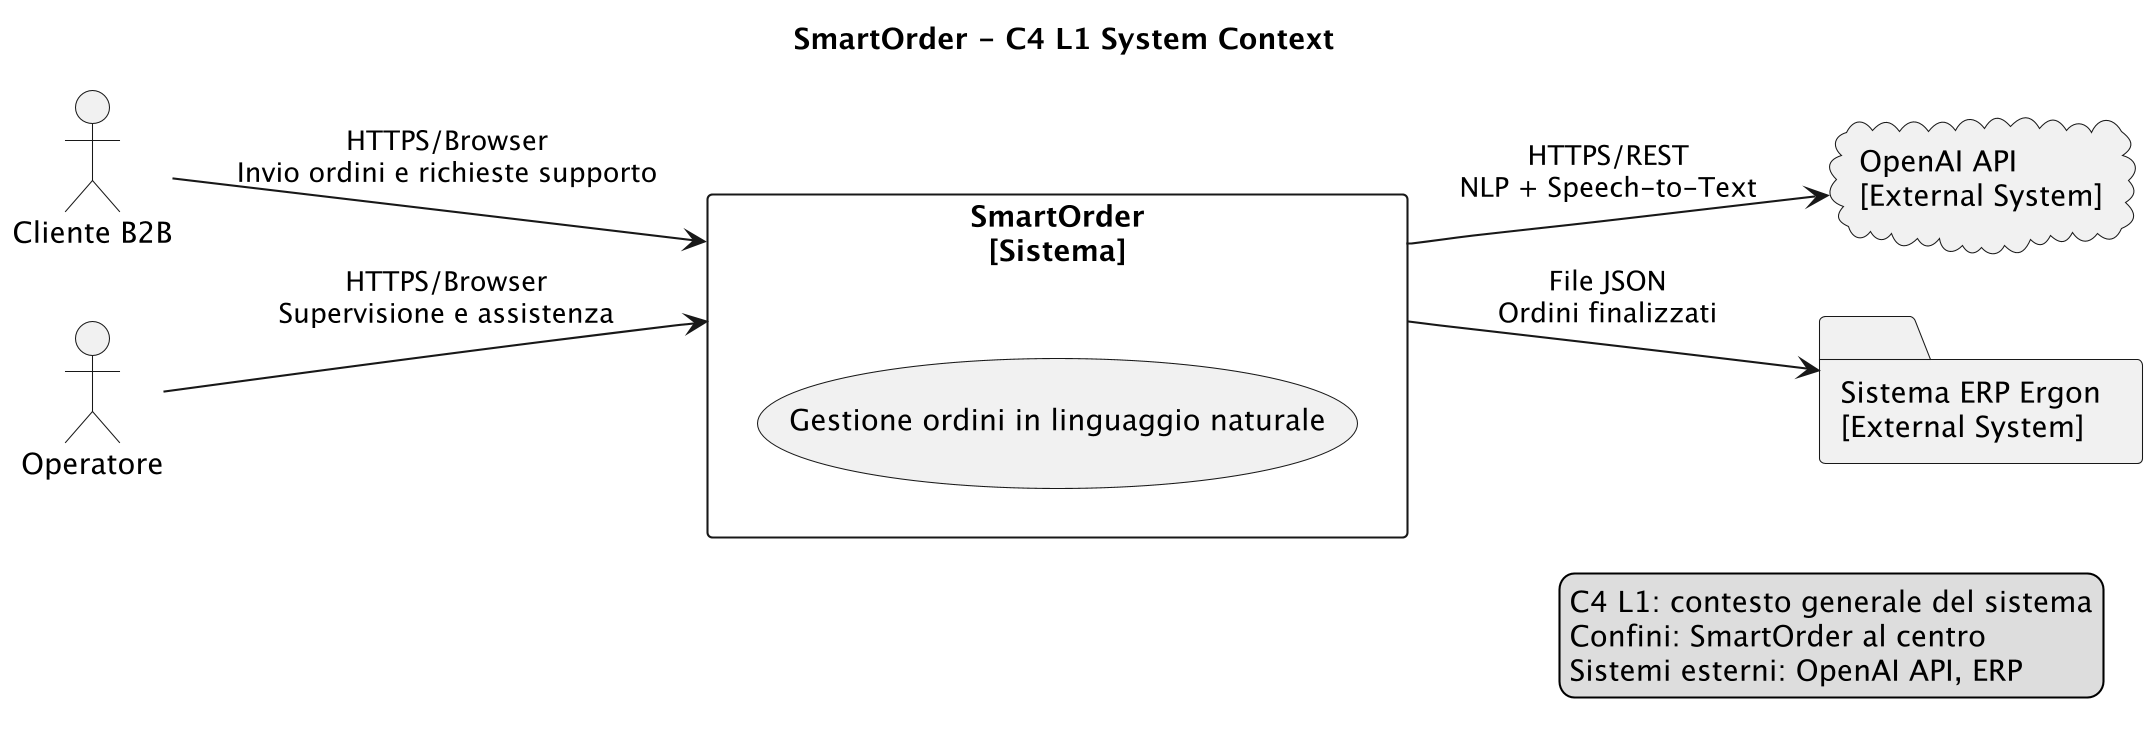
\includegraphics[width=0.95\textwidth]{arch_c4_l1_context.png}
    \caption{Diagramma C4 L1 (PlantUML compilato): contesto del sistema SmartOrder.}
\end{figure}

\begin{table}[H]
    \centering
    \renewcommand{\arraystretch}{1.2}
    \begin{tabularx}{\textwidth}{@{}lL@{}}
        \toprule
        \textbf{Elemento} & \textbf{Ruolo nel contesto} \\
        \midrule
        Cliente & Agente commerciale B2B che inserisce ordini in linguaggio naturale e richiede assistenza. \\
        Operatore & Utente interno che supervisiona ticket, casi a bassa confidence e correzioni AI. \\
        SmartOrder & Sistema oggetto della specifica; acquisisce input multimodale e genera ordini strutturati. \\
        OpenAI API & Servizio esterno usato per comprensione linguaggio naturale e trascrizione audio. \\
        Sistema ERP & Gestionale aziendale che riceve ordini finalizzati in formato JSON. \\
        \bottomrule
    \end{tabularx}
    \caption{C4 L1 - Contesto del sistema SmartOrder.}
\end{table}

\subsection{Vista C4 - Livello 2 (Container)}
Il diagramma C4 Livello 2 (pagina \texttt{C4L2}) decompone SmartOrder nei container applicativi principali.

\begin{figure}[H]
    \centering
    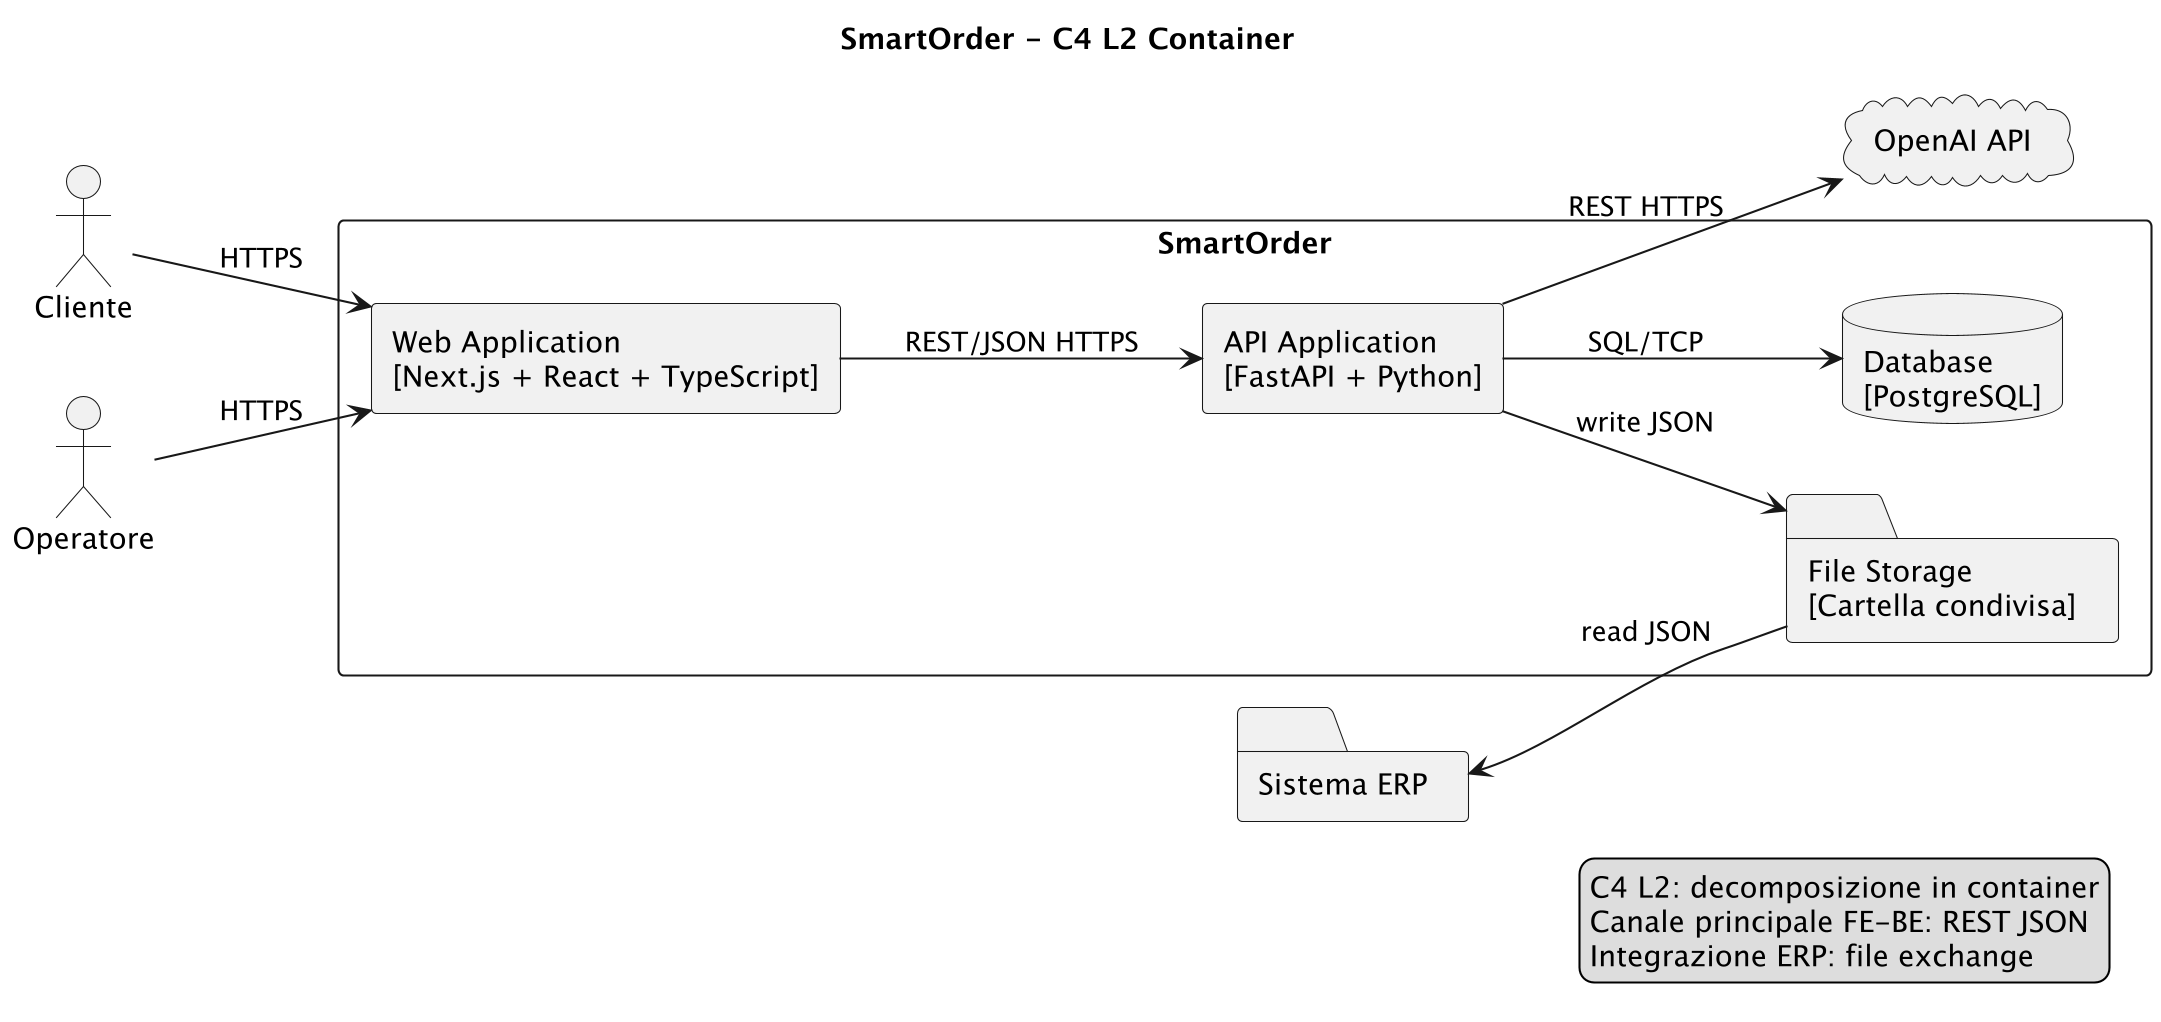
\includegraphics[width=0.95\textwidth]{arch_c4_l2_container.png}
    \caption{Diagramma C4 L2 (PlantUML compilato): vista container.}
\end{figure}

\begin{table}[H]
    \centering
    \renewcommand{\arraystretch}{1.2}
    \begin{tabularx}{\textwidth}{@{}lL@{}}
        \toprule
        \textbf{Container} & \textbf{Responsabilita} \\
        \midrule
        Web Application (Next.js + React + TypeScript) & Interfaccia cliente/operatore, gestione sessione utente, rendering chat, carrello, storico, dashboard operative. \\
        API Application (FastAPI) & Business logic di dominio: autenticazione, orchestrazione AI, gestione carrello/ordini/ticket, persistenza e pubblicazione output. \\
        Database (PostgreSQL) & Persistenza strutturata di utenti, sessioni, carrelli, ordini, ticket, log AI e catalogo. \\
        File Storage (cartella condivisa) & Punto di consegna ordini finalizzati in JSON verso processo ERP esterno. \\
        \bottomrule
    \end{tabularx}
    \caption{C4 L2 - Container e responsabilita.}
\end{table}

\subsection{Stile architetturale adottato}
La soluzione adotta uno stile \textbf{client-server a servizi}, con frontend e backend separati e API REST come contratto principale.
All'interno del backend viene applicata una suddivisione per layer logici (Controller, Application Service, Core Domain, Outbound Ports) coerente con i principi di \textit{Ports and Adapters}.

Le principali motivazioni della scelta sono:
\begin{itemize}
    \item isolamento della logica di business da dipendenze infrastrutturali;
    \item testabilita delle regole applicative in assenza di interfaccia grafica;
    \item sostituibilita di adapter esterni (servizi AI, storage, connettori DB) con impatto ridotto;
    \item evoluzione indipendente dei rilasci frontend e backend.
\end{itemize}

% ===================================================================
%  6. ARCHITETTURA DI DEPLOYMENT
% ===================================================================
\newpage
\section{Architettura di deployment}

Questa sezione descrive la distribuzione fisica dei componenti del sistema \textit{SmartOrder}, illustrando gli ambienti di esecuzione, i nodi infrastrutturali coinvolti e le strategie di Continuous Integration e Continuous Deployment (CI/CD) adottate.

\subsection{Scenario di esecuzione}
Il sistema prevede due configurazioni principali per l'esecuzione, pensate per separare l'ambiente di sviluppo da quello di produzione:
\begin{itemize}
    \item \textbf{Ambiente di Sviluppo (Locale)}: i servizi di frontend e backend vengono eseguiti localmente sulla macchina di sviluppo, sfruttando la containerizzazione (es. Docker Compose) o task eseguiti in locale per avviare l'applicativo e un database PostgreSQL isolato. Questo garantisce un ambiente di test riproducibile.
    \item \textbf{Ambiente di Produzione (Cloud)}: l'intero applicativo è ospitato sulla piattaforma cloud \textbf{Railway}. Railway gestisce nativamente il provisioning delle risorse, ospitando in container isolati i servizi di frontend (Next.js), backend (FastAPI) e il database relazionale (PostgreSQL).
\end{itemize}

\subsection{Nodi e responsabilità di deployment}
La seguente vista descrive la mappatura tra i container software e le risorse cloud che li ospitano in ambiente di produzione.

\begin{figure}[H]
    \centering
    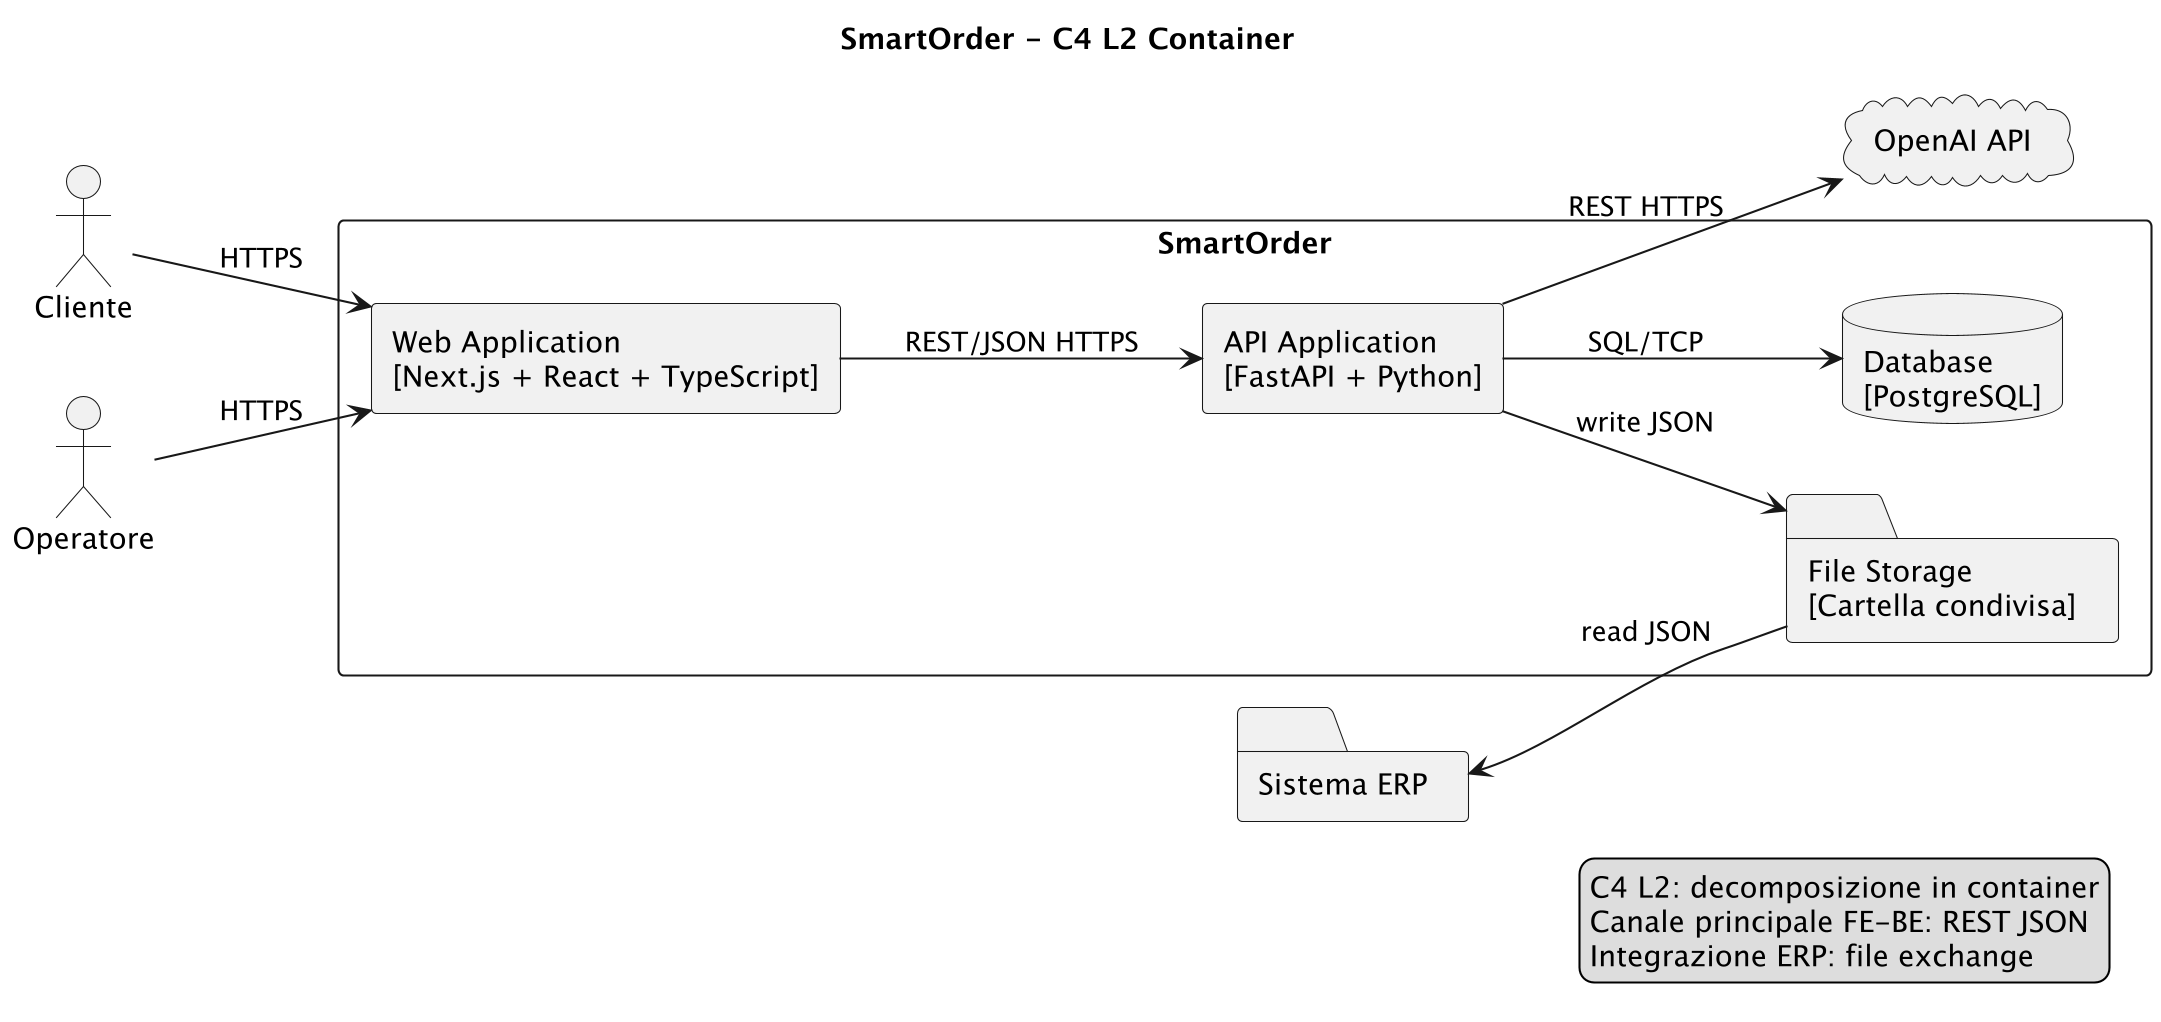
\includegraphics[width=0.95\textwidth]{arch_c4_l2_container.png}
    \caption{Vista di deployment logico del sistema.}
\end{figure}

\begin{table}[H]
    \centering
    \renewcommand{\arraystretch}{1.5}
    \begin{tabularx}{\textwidth}{@{}lX@{}}
        \toprule
        \textbf{Nodo Cloud} & \textbf{Responsabilità} \\
        \midrule
        \textbf{Frontend Service} \newline (Railway) & Espone la web application in Next.js tramite protocollo HTTPS. Gestisce il rendering dell'interfaccia utente, l'idratazione lato client e inoltra le richieste API verso il backend. \\
        \textbf{Backend Service} \newline (Railway) & Esegue il server Uvicorn con l'applicazione FastAPI. Centralizza la logica di business, l'orchestrazione delle chiamate AI e la validazione transazionale degli ordini. \\
        \textbf{Database Service} \newline (Railway PostgreSQL) & Istanza cloud gestita di PostgreSQL. Conserva i dati transazionali (utenti, ordini, carrelli, ticket) garantendo integrità, persistenza e backup continui. \\
        \textbf{File Storage Condiviso} \newline (Object Storage S3) & Bucket cloud (es. Amazon S3 o compatibile) utilizzato come buffer di integrazione aziendale. Il backend vi deposita i file JSON degli ordini finalizzati, i quali vengono successivamente prelevati dal sistema ERP esterno. \\
        \textbf{OpenAI Cloud API} \newline (Servizio Esterno) & Endpoint gestiti direttamente da OpenAI, richiamati dal backend per i servizi di Natural Language Processing (GPT-4o) e di speech-to-text (Whisper). \\
        \bottomrule
    \end{tabularx}
    \caption{Nodi logici di deployment e relative responsabilità.}
\end{table}

\textit{Nota architetturale sullo Storage Condiviso:} Per l'integrazione con l'ERP aziendale si è scelto di adottare un \textbf{Object Storage}. Rispetto a una semplice cartella di rete, un bucket cloud offre standard di sicurezza enterprise, garantisce isolamento dei permessi e fornisce un facile accesso tramite API per il polling da parte di sistemi terzi.

\subsection{Canali di comunicazione}
Le comunicazioni tra i vari nodi del sistema avvengono esclusivamente tramite protocolli sicuri e standardizzati:
\begin{itemize}
    \item \textbf{Frontend $\leftrightarrow$ Backend}: le chiamate API avvengono su canale cifrato HTTPS, scambiando payload in formato JSON. L'autenticazione è garantita tramite token o cookie di sessione sicuri.
    \item \textbf{Backend $\leftrightarrow$ PostgreSQL}: connessione su protocollo TCP proprietario del database, ottimizzata tramite un meccanismo di \textit{connection pooling} (gestito tramite \texttt{psycopg2}) per sopportare picchi di traffico.
    \item \textbf{Backend $\leftrightarrow$ OpenAI API}: invocazioni REST su rete pubblica cifrata HTTPS verso i server cloud di OpenAI.
    \item \textbf{Backend $\rightarrow$ File Storage}: scritture nel bucket cloud tramite chiamate API autenticate, necessarie a depositare l'ordine json per il sistema ERP.
\end{itemize}

\subsection{Aspetti operativi e CI/CD}
Per garantire rilasci continui, controllati e privi di disservizi, il progetto adotta pratiche automatizzate di \textit{Continuous Integration} e \textit{Continuous Deployment} (CI/CD):
\begin{itemize}
    \item \textbf{Continuous Integration (CI)}: grazie a \textit{GitHub Actions}, all'apertura di ogni Pull Request o push sui rami principali viene triggerato un workflow di controllo qualità (es. linter tramite ESLint) per prevenire il rilascio di codice formalmente scorretto.
    \item \textbf{Continuous Deployment (CD) automatizzato}: il deployment in produzione è delegato a \textbf{Railway}, il quale è interfacciato direttamente al repository GitHub. Ad ogni push sul branch principale, Railway rileva automaticamente i cambiamenti e lancia il processo di build e deploy. Questo avviene in modalità \textit{zero-downtime}, aggiornando i container senza causare interruzioni agli utenti.
    \item \textbf{Gestione dei Segreti}: chiavi API, credenziali del database e secret di cifratura non vengono mai committati nel repository. Sono configurati come variabili d'ambiente (Environment Variables) criptate direttamente all'interno della dashboard del progetto su Railway.
\end{itemize}

% ===================================================================
%  7. DESIGN PATTERN
% ===================================================================

\newpage
\section{Design pattern}

Questa sezione descrive i principali pattern architetturali e progettuali (ispirati alle soluzioni della \textit{Gang of Four} e ai pattern enterprise) adottati per risolvere problemi ricorrenti nel sistema \textit{SmartOrder}, sia lato backend che lato frontend.

% -------------------------------------------------------------------
\subsection{Dependency Injection}

\subsubsection{Descrizione del pattern}
La Dependency Injection è un pattern strutturale che implementa l'Inversione del Controllo (IoC). Consiste nel fornire le dipendenze (oggetti o servizi) a una classe dall'esterno, anziché lasciare che sia la classe stessa a istanziarle internamente.

\subsubsection{Motivazioni dell'utilizzo del pattern}
L'obiettivo principale è il disaccoppiamento dei componenti. Iniettando le dipendenze si rispetta il principio di Inversione delle Dipendenze (la "D" dei principi SOLID), rendendo il codice estremamente più modulare. Questo risulta fondamentale per la testabilità del sistema: permette infatti di iniettare agilmente dei \textit{mock} o \textit{stub} al posto dei servizi reali durante l'esecuzione degli unit test.

\subsubsection{Utilizzo del pattern nel progetto}
Il pattern è applicato in modo sistematico nel backend FastAPI. I controller del Livello 1 (Inbound Ports), come il \texttt{ConversationController} o il \texttt{CartController}, non creano mai direttamente le istanze dei service. Al contrario, ricevono i servizi necessari (es. \texttt{ConversationService}, \texttt{CartService}) tramite il meccanismo nativo di iniezione delle dipendenze del framework.

% -------------------------------------------------------------------
\subsection{Adapter (Ports and Adapters)}

\subsubsection{Descrizione del pattern}
L'Adapter è un pattern strutturale che permette a due interfacce incompatibili di collaborare. Agisce come un "traduttore" o un "ponte", incapsulando la logica di un sistema esterno e offrendo un'interfaccia compatibile con il dominio interno dell'applicazione.

\subsubsection{Motivazioni dell'utilizzo del pattern}
In un'architettura di tipo \textit{Ports and Adapters} (Architettura Esagonale), questo pattern è cruciale per isolare la logica di business (il "Core") dalle dipendenze tecnologiche esterne. Evita che i dettagli di librerie di terze parti o SDK "inquinino" il dominio applicativo, permettendo di sostituire un fornitore di servizi in futuro modificando solo l'Adapter, senza toccare le regole di business.

\subsubsection{Utilizzo del pattern nel progetto}
Nel backend, il pattern si concretizza nel Livello 5 (Infrastructure Adapters). Interfacce come \texttt{IAIClient} fungono da porte in uscita (Outbound Ports). La classe \texttt{OpenAIAdapter} implementa questa interfaccia e agisce come Adapter verso le API esterne, traducendo le entità del dominio di SmartOrder in formato JSON/REST specifico richiesto dai server di OpenAI, proteggendo il resto del sistema dai dettagli della libreria esterna.

% -------------------------------------------------------------------
\subsection{Repository Pattern}

\subsubsection{Descrizione del pattern}
Il Repository è un pattern architetturale (di livello enterprise) che media tra la logica di dominio e il layer di data mapping. Fornisce un'interfaccia che simula una collezione di oggetti in memoria, nascondendo le complessità legate all'estrazione e al salvataggio dei dati persistenti.

\subsubsection{Motivazioni dell'utilizzo del pattern}
L'utilizzo del Repository centralizza l'accesso al database, evitando la frammentazione delle query SQL all'interno della logica di business. Garantisce un singolo punto di verità per le operazioni CRUD, semplifica la manutenzione del codice legato alla persistenza e facilita eventuali migrazioni tecnologiche.

\subsubsection{Utilizzo del pattern nel progetto}
Nel backend, l'interazione con il database relazionale (PostgreSQL) è astratta attraverso le interfacce definite nel Livello 4 (Outbound Ports) come \texttt{IUserRepository}, \texttt{IOrderRepository} e \texttt{ITicketRepository}. L'implementazione pratica di queste interfacce è delegata all'infrastruttura sottostante (come \texttt{PostgresAdapter} o \texttt{IDBSessionManager}), in modo che i servizi applicativi lavorino unicamente con oggetti di dominio.

% -------------------------------------------------------------------
\subsection{Facade}

\subsubsection{Descrizione del pattern}
Il Facade è un pattern strutturale che fornisce un'interfaccia unificata, astratta e semplificata a un insieme di interfacce o moduli più complessi all'interno di un sottosistema, nascondendone i dettagli di basso livello.

\subsubsection{Motivazioni dell'utilizzo del pattern}
Il pattern riduce l'accoppiamento tra i client e il sottosistema complesso, offrendo un punto di accesso centralizzato e facile da usare. Questo migliora la leggibilità del codice, agevola lo sviluppo e riduce la curva di apprendimento per i componenti che devono interfacciarsi con logiche articolate.

\subsubsection{Utilizzo del pattern nel progetto}
Nel frontend React/Next.js, i moduli presenti nel Livello 3 (Service Layer API Client), come \texttt{chatService}, \texttt{cartService} e \texttt{ticketService}, fungono da Facade verso la rete. Nascondono ai componenti visivi React l'intera complessità delle comunicazioni HTTP/REST verso FastAPI (iniezione dei token JWT negli header, gestione errori e serializzazione JSON), offrendo un'interfaccia pulita e semplice da invocare.

% -------------------------------------------------------------------
\subsection{Observer (State Management Reattivo)}

\subsubsection{Descrizione del pattern}
L'Observer è un pattern comportamentale che definisce una dipendenza uno-a-molti tra oggetti. Quando l'oggetto osservato (Subject) cambia stato, tutti gli oggetti dipendenti (Observer) vengono notificati e aggiornati automaticamente.

\subsubsection{Motivazioni dell'utilizzo del pattern}
Nel contesto dello sviluppo di interfacce utente, l'Observer è vitale per garantire che la UI rifletta sempre lo stato attuale dei dati senza dover implementare costosi meccanismi di polling. Permette di creare interfacce dinamiche e reattive in cui i componenti si limitano ad "ascoltare" le modifiche pertinenti.

\subsubsection{Utilizzo del pattern nel progetto}
Applicato nel frontend Next.js per la gestione dello stato globale al Livello 2. I vari Context Provider (es. \texttt{ChatContext}, \texttt{CartContext}, \texttt{NotificationContext}) assumono il ruolo di Subject, mantenendo la verità sui dati correnti. Event handler come \texttt{Chat Event Handler} o \texttt{Ticket Event Handler} ascoltano il \textit{RT Gateway} tramite WebSocket e aggiornano i contesti. I componenti grafici dell'interfaccia iscritti (Observer) vengono così notificati, innescando un re-render istantaneo della sola porzione interessata.

% ===================================================================
%  8. DATABASE
% ===================================================================
\newpage
\section{Database}

Questa sezione descrive l'architettura dei dati del sistema \textit{SmartOrder}, definendo il ruolo del database, le macro-aree informative gestite, i vincoli di integrità applicati e le modalità di interscambio dati con il sistema gestionale esterno.

\subsection{Ruolo del database nel sistema}
Il sistema si avvale di \textbf{PostgreSQL} (in hosting cloud su Railway) come unica fonte dati transazionale (Single Source of Truth) per il backend FastAPI. 
Il database relazionale assolve a tre ruoli fondamentali:
\begin{itemize}
    \item \textbf{Persistenza Transazionale:} memorizza in modo consistente lo stato delle sessioni, dei carrelli in lavorazione, dei ticket di assistenza e lo storico degli ordini consolidati.
    \item \textbf{Replica del Catalogo ERP:} ospita le tabelle anagrafiche dei prodotti e dei clienti sincronizzate dal gestionale aziendale, permettendo al sistema di operare con logiche di business locali (es. verifica assortimenti).
    \item \textbf{Motore di Ricerca Vettoriale:} tramite l'estensione \texttt{pgvector}, il database archivia gli \textit{embeddings} generati dai modelli LLM e risolve le query semantiche di "Vector Search", mappando le descrizioni in linguaggio naturale ai codici articolo reali.
\end{itemize}

\subsection{Macro-aree informative}
Il modello relazionale del database è logicamente suddiviso in macro-aree, ciascuna responsabile di un dominio specifico dell'applicazione.

\begin{table}[H]
    \centering
    \renewcommand{\arraystretch}{1.5}
    \begin{tabularx}{\textwidth}{@{}lX@{}}
        \toprule
        \textbf{Area Logica} & \textbf{Contenuto principale e Responsabilità} \\
        \midrule
        \textbf{Identità e Accesso} & Entità relative agli utenti, ruoli (Cliente, Operatore), credenziali crittografate (hash scrypt) e gestione dei token/sessioni attive. \\
        \textbf{Catalogo e Assortimento} & Anagrafica articoli (\texttt{anaart}), metadati descrittivi, \textit{embeddings} vettoriali per la ricerca semantica e tabelle di visibilità/assortimento per singolo cliente (\texttt{asscli}). \\
        \textbf{Carrello e Ordini} & Record transazionali che rappresentano il carrello corrente della sessione, le singole righe prodotto con le relative quantità e lo storico degli ordini finalizzati pronti per la consultazione (Storico Ordini). \\
        \textbf{Ticketing e Chat} & Entità per la gestione dell'assistenza (\textit{Human-in-the-loop}). Include i record dei Ticket (stati: "Aperto", "In lavorazione", "Chiuso"), l'assegnazione all'Operatore (Lock) e il tracciato cronologico (Log) dei messaggi di chat scambiati. \\
        \textbf{Log AI e Ottimizzazione} & Archiviazione diagnostica delle interazioni con il modello LLM. Comprende il \textit{Confidence Score}, i feedback degli utenti e le discrepanze generate dalle correzioni manuali ai carrelli, utili al \textit{retraining}. \\
        \bottomrule
    \end{tabularx}
    \caption{Aree logiche del modello dati relazionale.}
\end{table}

\subsection{Vincoli dati rilevanti}
Per garantire la robustezza del sistema e prevenire l'invio di ordini commercialmente invalidi al sistema ERP, il database impone rigorosi vincoli di integrità e di dominio:
\begin{itemize}
    \item \textbf{Vincolo di Assortimento (Foreign Key logica):} un prodotto può essere inserito nel carrello di una sessione solo se esiste una corrispondenza valida nella tabella degli assortimenti autorizzati (\texttt{asscli}) per il Cliente in esame.
    \item \textbf{Vincolo di Disponibilità:} controlli a livello database (\texttt{anaart}) impediscono l'immissione in ordine di articoli marcati con stato "sospeso" o "non disponibile".
    \item \textbf{Integrità Referenziale Standard:} chiavi esterne (Foreign Keys) con regole di propagazione \textit{ON DELETE CASCADE/RESTRICT} collegano indissolubilmente le righe dell'ordine all'ID Ordine padre e alla relativa anagrafica Cliente, prevenendo record orfani.
    \item \textbf{Vincolo di Quantità Commerciale:} i campi quantitativi delle righe ordine possiedono vincoli (\textit{CHECK constraints}) per impedire valori nulli, negativi o incompatibili con i multipli di vendita (es. logica a "casse").
\end{itemize}

\subsection{Output verso ERP}
Il database di SmartOrder funge da ambiente di \textit{staging} e composizione. Al termine del processo di checkout, i dati transazionali (intestazione ordine, righe, quantità e ID cliente) estratti dalle tabelle relazionali subiscono un processo di serializzazione. 

Il sistema genera un \textbf{payload strutturato in formato JSON} conforme al contratto di integrazione concordato con il fornitore del gestionale. Questo file non viene immagazzinato a lungo termine nel database cloud, ma viene immediatamente depositato nel \textbf{File Storage condiviso (Bucket S3)}, che rappresenta il reale punto di aggancio e consegna formale della transazione verso il sistema ERP aziendale.

% ===================================================================
%  9. ARCHITETTURA DI DETTAGLIO
% ===================================================================
\newpage
\section{Architettura di dettaglio}

\subsection{Frontend - C4 Livello 3 e 4}
Le pagine \texttt{C4L3F} e \texttt{C4L4F} descrivono una struttura a layer del frontend Next.js.

\begin{figure}[H]
    \centering
    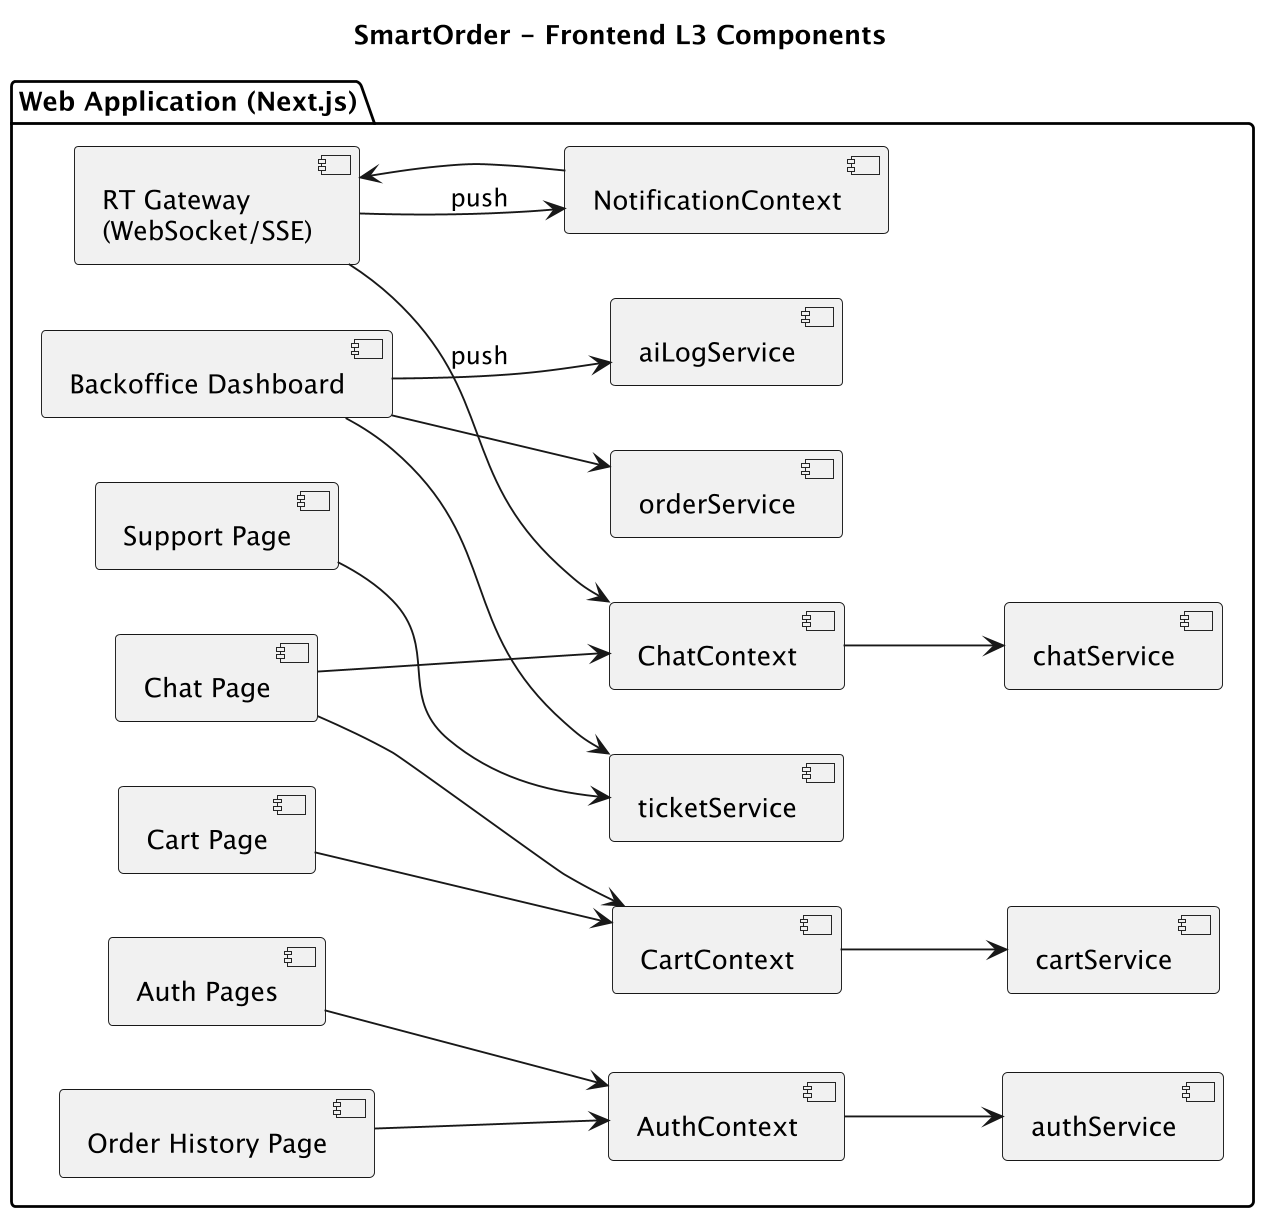
\includegraphics[width=0.98\textwidth]{arch_frontend_l3_components.png}
    \caption{Frontend L3 (PlantUML compilato): componenti principali.}
\end{figure}

\begin{figure}[H]
    \centering
    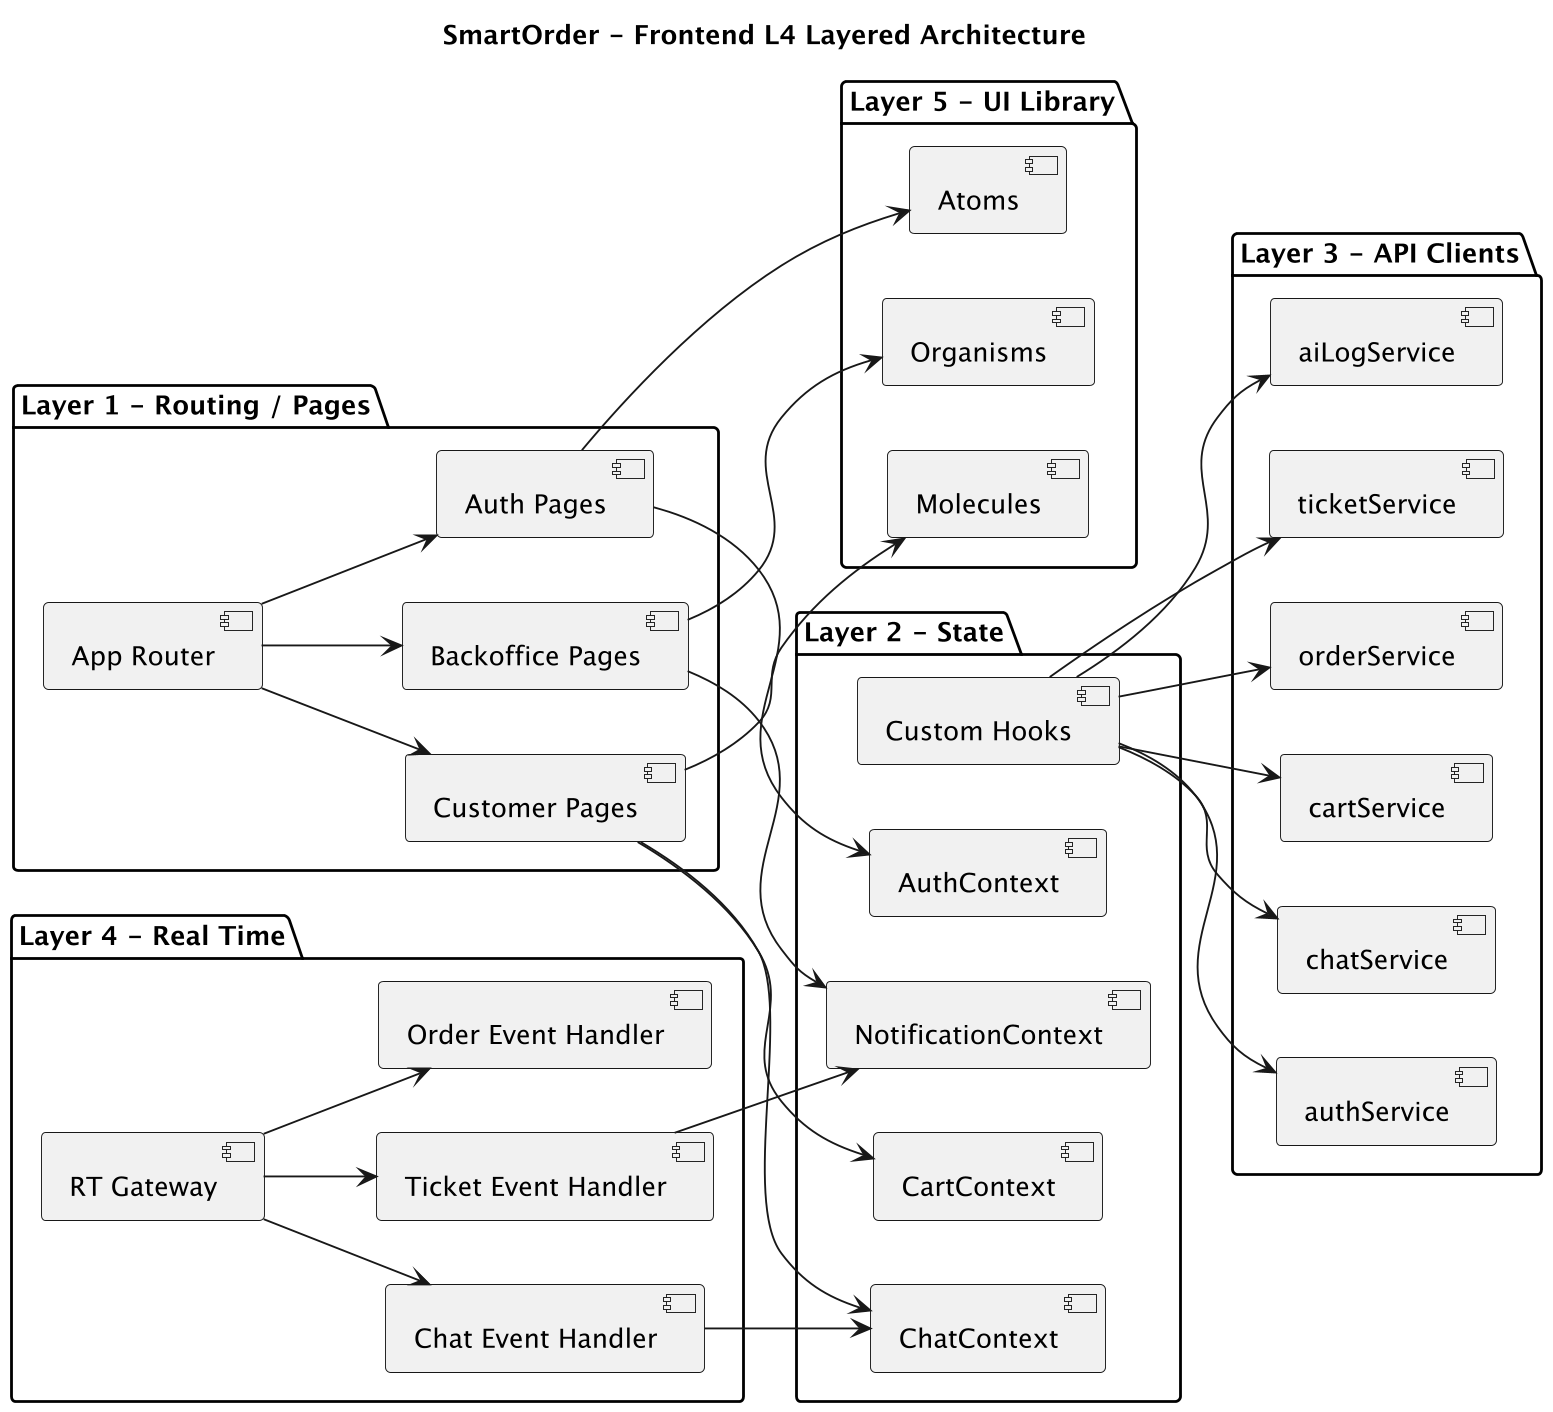
\includegraphics[width=0.98\textwidth]{arch_frontend_l4_layers.png}
    \caption{Frontend L4 (PlantUML compilato): layered architecture orientata al coding.}
\end{figure}

\subsubsection{Layer 1 - Routing e Pages}
Organizza route e viste principali:
\begin{itemize}
    \item area autenticazione (login, recupero password, profilo);
    \item area cliente (chat, carrello, storico, supporto);
    \item area operatore/backoffice (ticket, ordini globali, dashboard AI).
\end{itemize}

\subsubsection{Layer 2 - State Management}
Utilizza Context e custom hooks per stato condiviso:
\begin{itemize}
    \item \texttt{AuthContext}: identita e ruolo;
    \item \texttt{CartContext}: stato carrello e confidence score;
    \item \texttt{ChatContext}: messaggi live e modalita AI/Operatore;
    \item \texttt{NotificationContext}: eventi e notifiche applicative.
\end{itemize}

\subsubsection{Layer 3 - Service/API Client}
Ogni dominio espone un modulo dedicato (auth, cart, product, order, ticket, chat, ai-log) con responsabilita circoscritte e contratto REST verso backend.

\subsubsection{Layer 4 - Real-time}
Un gateway applicativo gestisce WebSocket/SSE e aggiorna in push chat, ticket, ordini e log AI.

\subsubsection{Layer 5 - UI Library}
Componenti organizzati secondo \textit{Atomic Design} (atoms, molecules, organisms) per uniformare esperienza utente tra aree cliente e operatore.

\subsection{Backend - C4 Livello 3 e 4}
Le pagine \texttt{C4L3B} e \texttt{C4L4B} rappresentano la decomposizione interna del container FastAPI.

\begin{figure}[H]
    \centering
    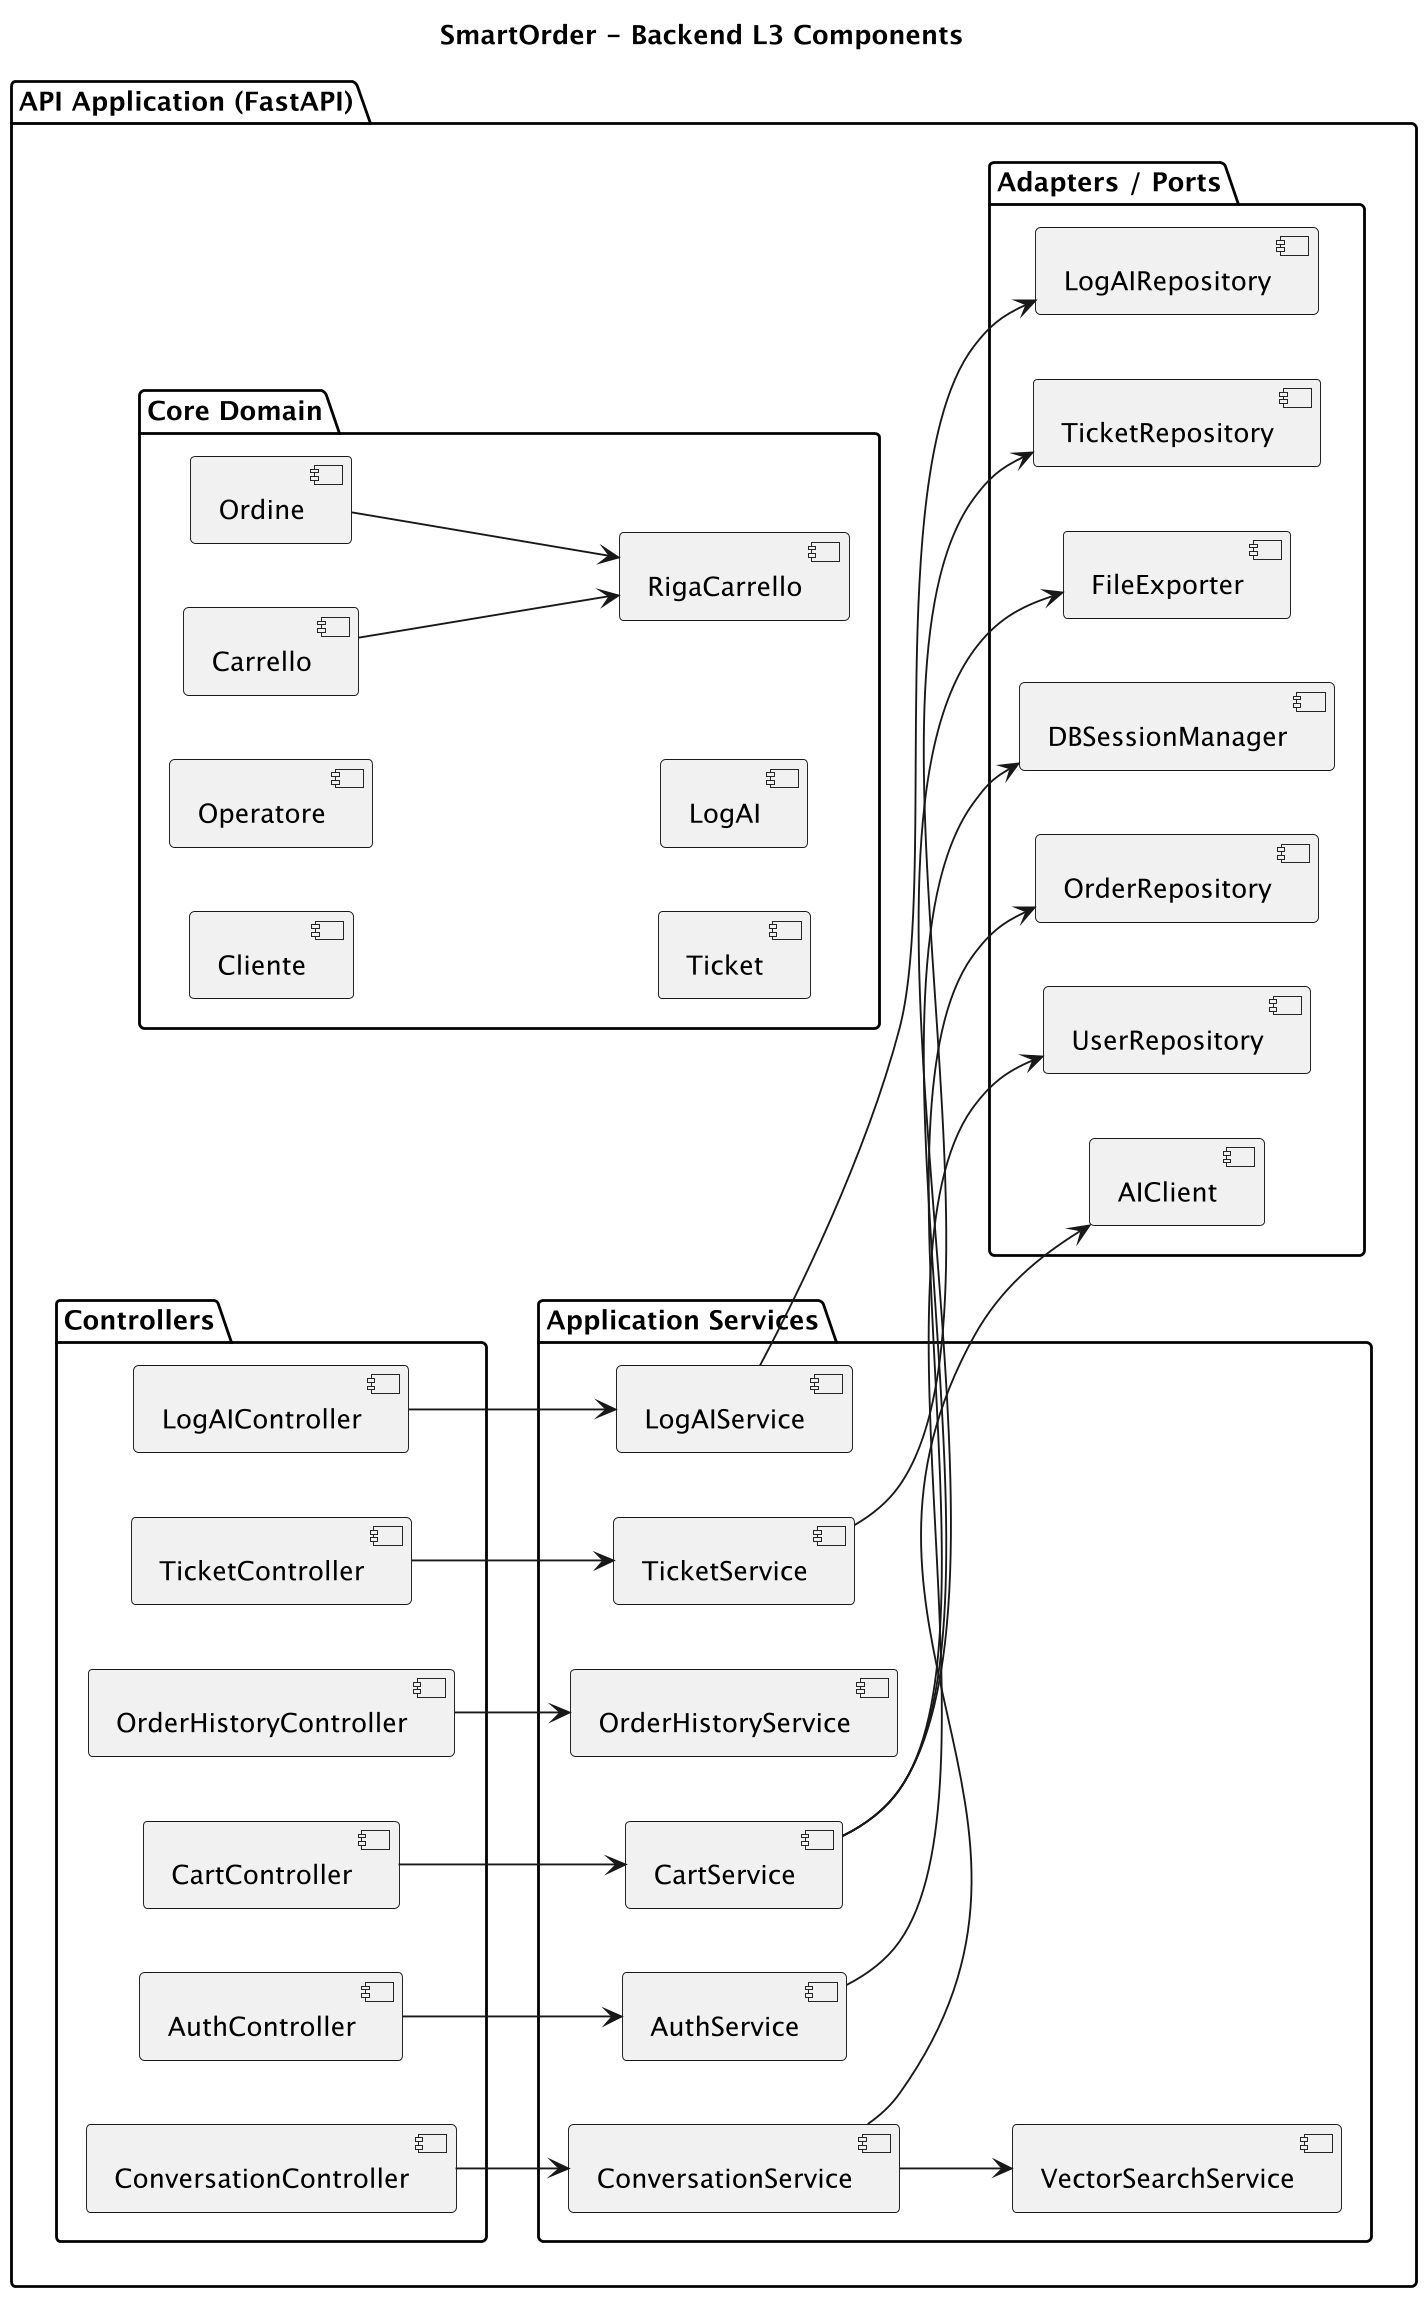
\includegraphics[width=0.98\textwidth]{arch_backend_l3_components.png}
    \caption{Backend L3 (PlantUML compilato): componenti applicativi e dipendenze.}
\end{figure}

\begin{figure}[H]
    \centering
    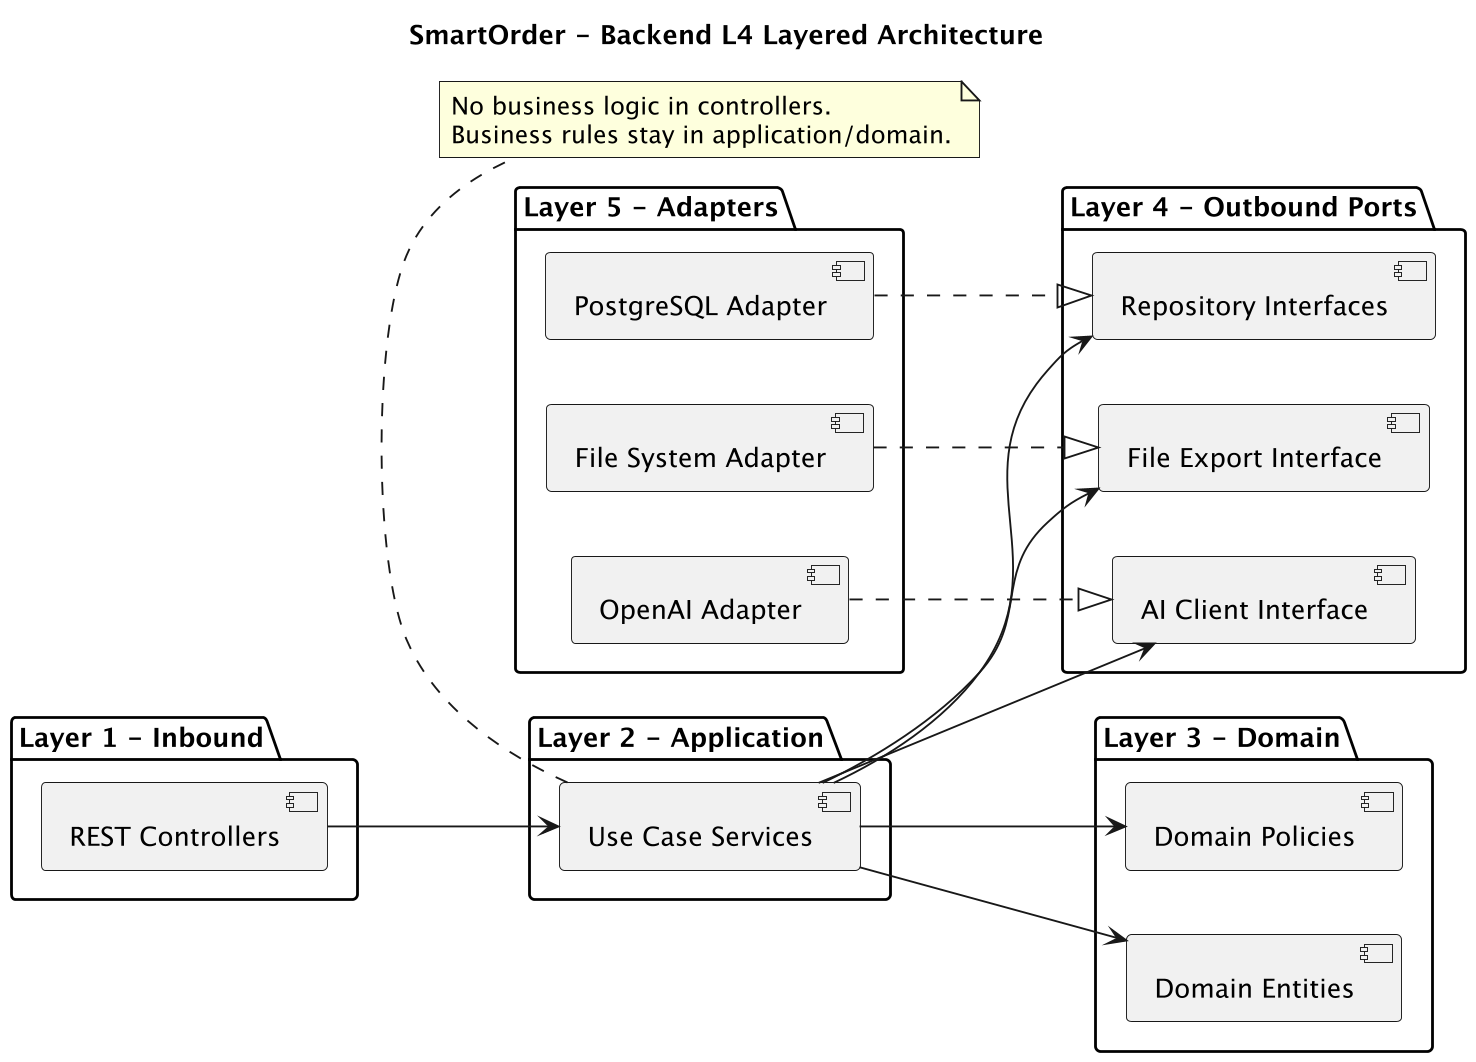
\includegraphics[width=0.98\textwidth]{arch_backend_l4_layers.png}
    \caption{Backend L4 (PlantUML compilato): layer, ports e adapters.}
\end{figure}

\subsubsection{Controllers (Inbound Ports)}
Punto di ingresso HTTP per i principali domini:
\texttt{AuthController}, \texttt{ConversationController}, \texttt{CartController}, \texttt{OrderHistoryController}, \texttt{TicketController}, \texttt{LogAIController}.

\subsubsection{Application Services (Use Cases)}
Orchestrano regole e collaborazioni tra moduli:
\texttt{AuthService}, \texttt{ConversationService}, \texttt{CartService}, \texttt{OrderHistoryService}, \texttt{VectorSearchService}, \texttt{TicketService}, \texttt{LogAIService}.

\subsubsection{Core Domain}
Entita principali del dominio applicativo: Cliente, Operatore, Carrello, RigaCarrello, Ordine, Ticket, LogAI.

\begin{figure}[H]
    \centering
    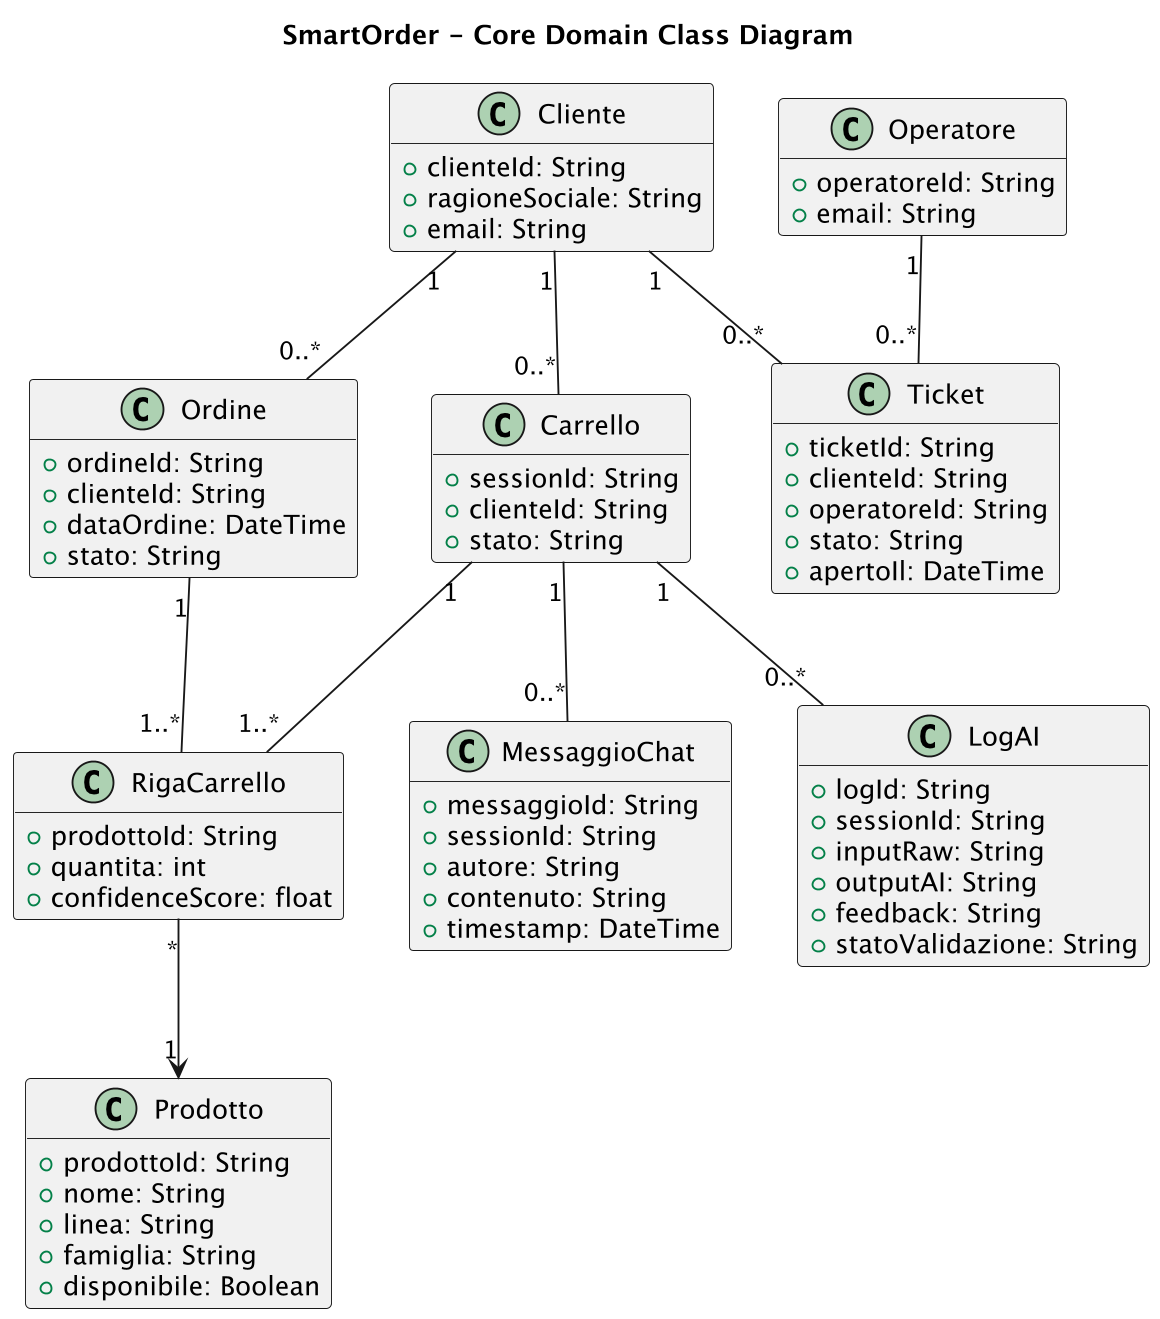
\includegraphics[width=0.95\textwidth]{arch_domain_class_core.png}
    \caption{Core Domain (PlantUML compilato): classi principali e relazioni.}
\end{figure}

\subsubsection{Outbound Ports e Adapter}
Interfacce astratte per dipendenze esterne:
\begin{itemize}
    \item repository dati (utenti, ordini, ticket, log);
    \item manager sessioni DB;
    \item client AI verso OpenAI;
    \item exporter file JSON per integrazione ERP.
\end{itemize}

\subsection{Flusso applicativo principale (ordine)}
\begin{enumerate}
    \item Il Cliente invia input naturale (testo/audio/immagine) dalla Chat Page.
    \item Il backend interpreta input e aggiorna il carrello con confidence score associato.
    \item Il Cliente (o Operatore in delega) conferma il checkout del carrello.
    \item Il backend valida vincoli (assortimento/disponibilita), persiste l'ordine e genera JSON.
    \item Il file JSON viene depositato in storage condiviso per acquisizione ERP.
\end{enumerate}

\begin{figure}[H]
    \centering
    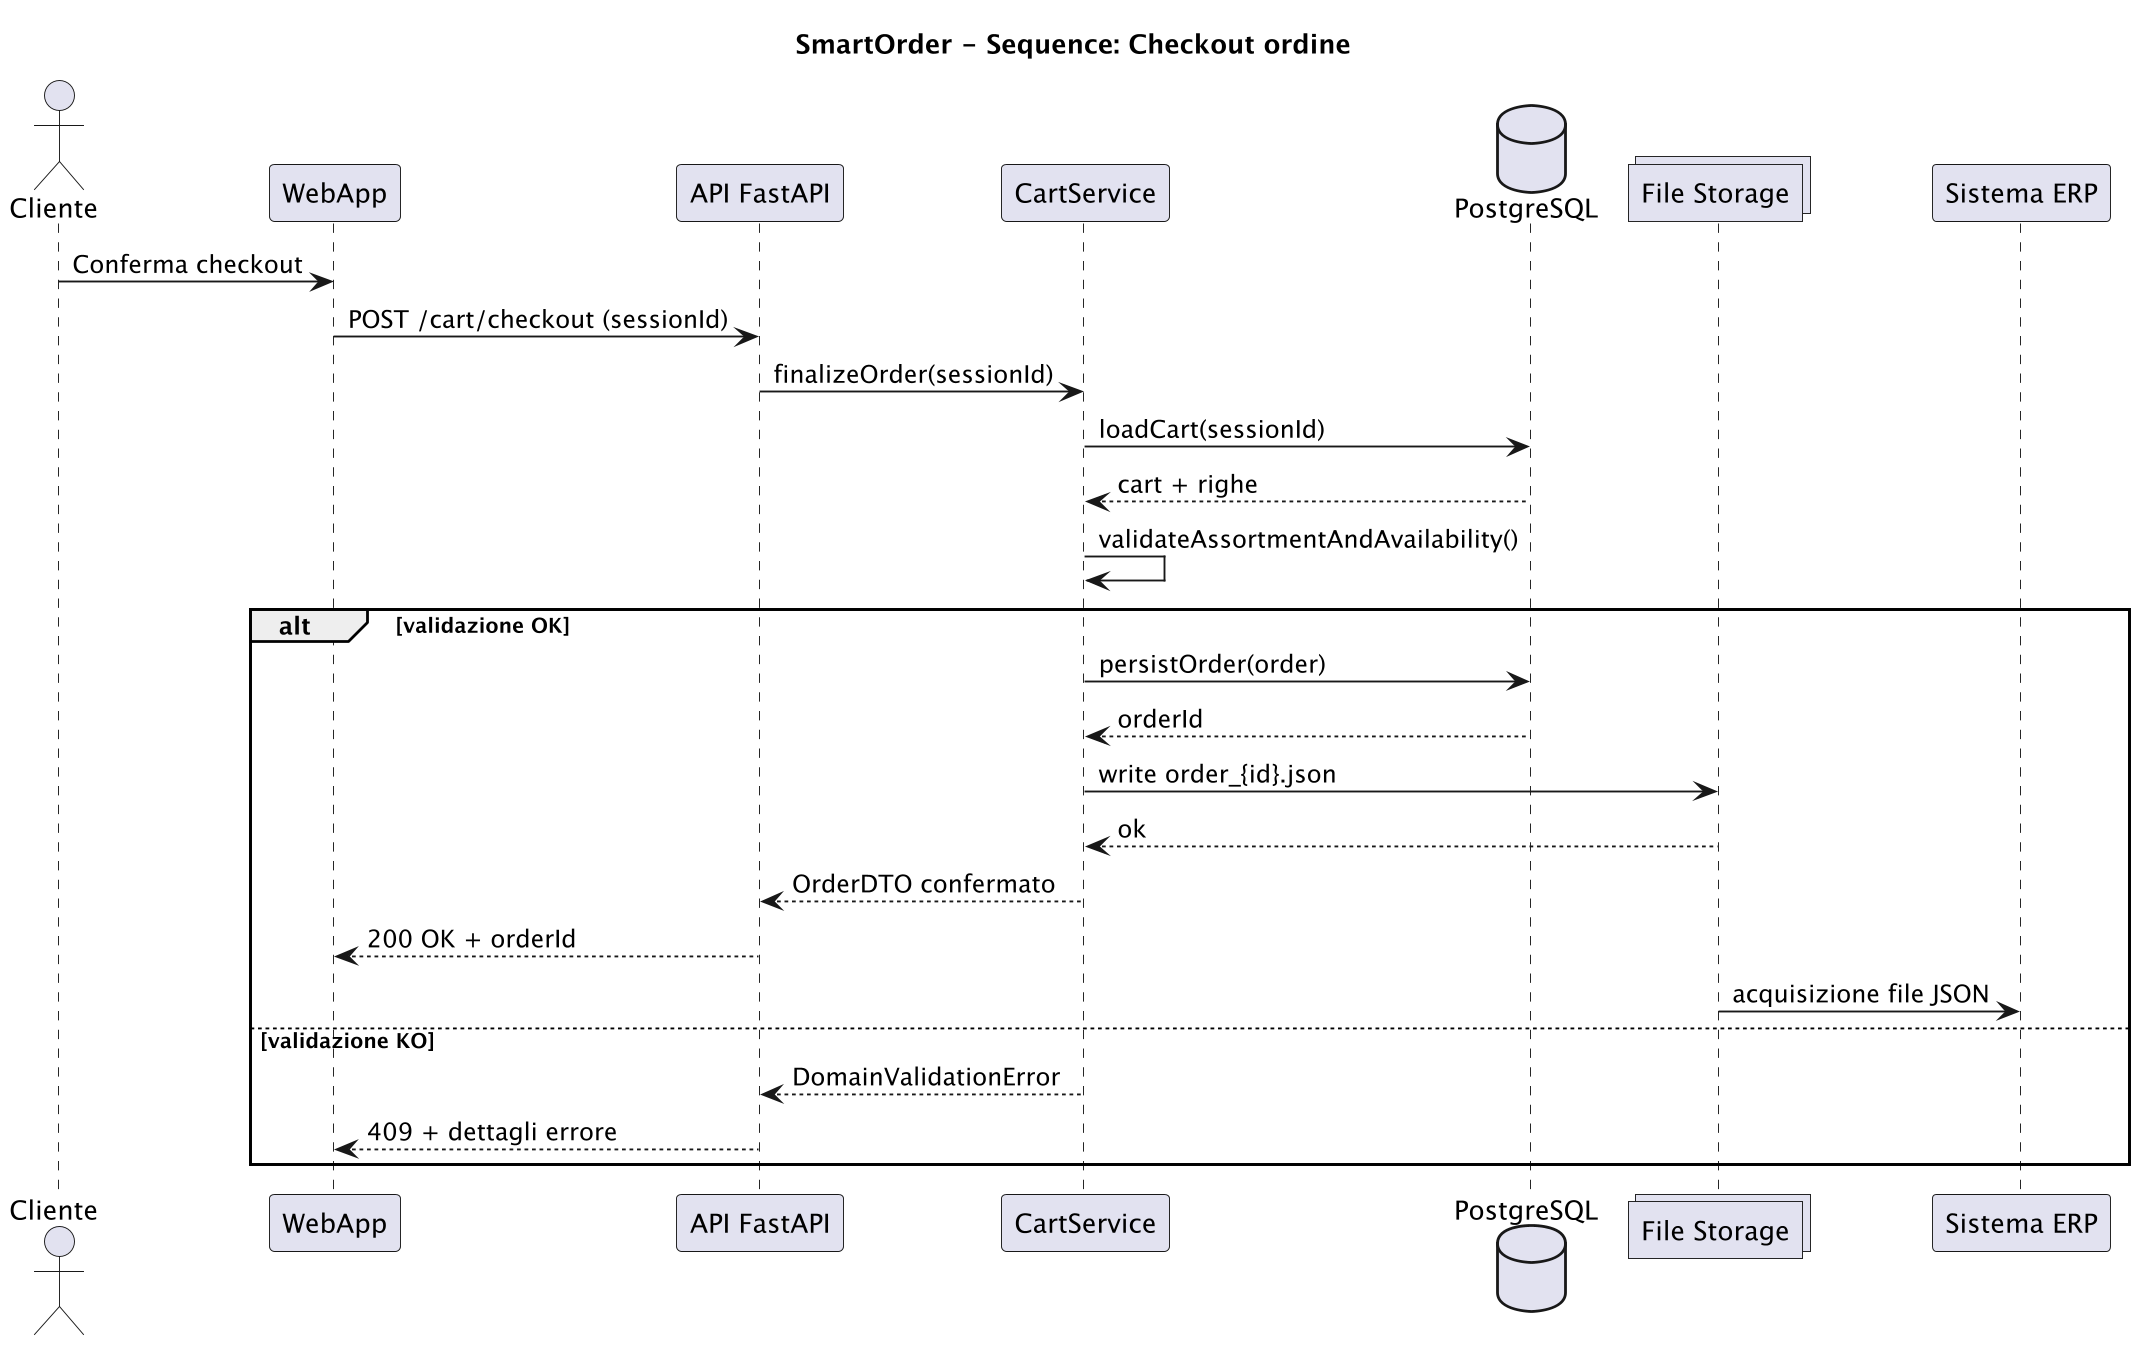
\includegraphics[width=0.98\textwidth]{arch_sequence_checkout.png}
    \caption{Flusso checkout (PlantUML compilato): sequenza end-to-end.}
\end{figure}

% ===================================================================
%  10. SORGENTI PLANTUML
% ===================================================================
\newpage
\section{Sorgenti PlantUML}

Questa sezione elenca i sorgenti \texttt{.puml} ufficiali da usare per generare i diagrammi architetturali.
Per ogni sorgente viene mantenuto anche l'output compilato in formato \texttt{.png}, cosi da poter includere direttamente le figure nel documento.
I file sono mantenuti nella directory \texttt{Contenuti/} e versionati insieme alla specifica.

\begin{table}[H]
    \centering
    \renewcommand{\arraystretch}{1.2}
    \begin{tabularx}{\textwidth}{@{}l l L@{}}
        \toprule
        \textbf{File \texttt{.puml}} & \textbf{Output \texttt{.png}} & \textbf{Contenuto} \\
        \midrule
        \texttt{arch\_c4\_l1\_context.puml} & \texttt{arch\_c4\_l1\_context.png} & C4 Livello 1: attori esterni, sistema SmartOrder, sistemi terzi. \\
        \texttt{arch\_c4\_l2\_container.puml} & \texttt{arch\_c4\_l2\_container.png} & C4 Livello 2: WebApp, API, DB, File Storage, OpenAI, ERP. \\
        \texttt{arch\_frontend\_l3\_components.puml} & \texttt{arch\_frontend\_l3\_components.png} & C4 Livello 3 frontend: pagine, context, servizi API client, real-time. \\
        \texttt{arch\_backend\_l3\_components.puml} & \texttt{arch\_backend\_l3\_components.png} & C4 Livello 3 backend: controller, service, core, adapter. \\
        \texttt{arch\_frontend\_l4\_layers.puml} & \texttt{arch\_frontend\_l4\_layers.png} & Livello 4 frontend: layered architecture per coding guidato. \\
        \texttt{arch\_backend\_l4\_layers.puml} & \texttt{arch\_backend\_l4\_layers.png} & Livello 4 backend: layer applicativi e dipendenze interne. \\
        \texttt{arch\_domain\_class\_core.puml} & \texttt{arch\_domain\_class\_core.png} & Diagramma classi del core domain (entita e relazioni). \\
        \texttt{arch\_sequence\_checkout.puml} & \texttt{arch\_sequence\_checkout.png} & Diagramma di sequenza del flusso principale di checkout. \\
        \bottomrule
    \end{tabularx}
    \caption{Elenco sorgenti PlantUML e output compilati dell'architettura.}
\end{table}

\subsection{Convenzioni operative}
\begin{itemize}
    \item ogni file PlantUML deve essere modificabile senza dipendere da asset esterni;
    \item i nomi dei componenti devono essere allineati ai nomi usati nella sezione 9;
    \item ogni diagramma include titolo, legenda minima e protocollo principale tra componenti;
    \item i diagrammi L4 sono orientati alla codifica (classi, package, dipendenze).
\end{itemize}

\end{document}
